% typ dokumentu,draft
\documentclass[12pt,twoside]{article}

% użycie pakietu , jak include
\usepackage{weiiszablon}

% autor pracy
\author{Krystian Olszowy}

% np. EF-123456, EN-654321, ..., Numer albumu
\studentID{EA-167582}

\title{Aplikacja na smartfony do sterowania telewizorem}
\titleEN{{Mobile application for controlling TV set}}


%%% wybierz rodzaj pracy wpisując jeden z poniższych numerów: ...
% 1 = inżynierska	% BSc
% 2 = magisterska	% MSc
% 3 = doktorska		% PhD
%%% na miejsce zera w linijce poniżej
\newcommand{\rodzajPracyNo}{1}


%%% promotor
\supervisor{dr inż. Jan Sadolewski}
%% przykład: dr hab. inż. Józef Nowak, prof. PRz

%%% promotor ze stopniami naukowymi po angielsku
\supervisorEN{Jan Sadolewski, PhD, Eng.}

\abstract{Treść streszczenia po polsku}
\abstractEN{Treść streszczenia po angielsku}

\keywords{pilot, BLE, IR, Flutter, aplikacja mobilna}
\keywordsEN{remote controller, BLE, IR, Flutter, mobile application}


\begin{document}

% strona tytułowa
\maketitle

\blankpage

% spis treści
\tableofcontents

\clearpage
\blankpage

\section{Wstęp}
\subsection{Telewizor i sposoby sterowania nim}
Współcześnie nie wyborażamy sobie domu, w którym nie ma telewizora. Telewizory, będące
centralnym elementem więszkości domostw, przekształciły się z tradycyjnych urządzeń
telewizyjnych w zaawansowane systemy multimedialne, oferujące nie tylko dostęp do programów telewizyjnych,
ale również do różnorodnych treści wideo, gier, czy nawet aplikacji internetowych.
Ich powszechność we współczesnym świecie, a także mnogość producentów i ich pomysłów
sprawiło, że wyodrębniło się wiele technologii i sposobów sterowania tymi urządzeniami.

W wielu gospodarstwach domowych znajduje się wciąż telewizor sterowany jedynie za pomocą podczerwieni i jest
to nadal najpopularniejszy sposób sterowania tymi urzadzeniami. Rozwiązania takie jak sterowanie poprzez WiFi, czy Bluetooth
mimo, że są już pewien czas na rynku, jeszcze nie goszczą u wszystkich użytkowników. Jest tak zazwyczaj z powodu ceny
nowego urządzenia multimedialnego lub zwykłego braku potrzeby wymiany telewizora. Czy jest jednak sposób aby
móc korzystać z wygody nowych rozwiązań komunikacji bezprzewodowej oraz mieć urządzenie zdolne do sterowania
telewizorem zawsze w naszej kieszeni, wspierające urządzenia telewizyjne nie posiadające obsługi nowoczesnych technologii bezprzewodowych?

\subsection{Smartfon i jego powszechność}
W dynamicznie rozwijającym się świecie, smartfony stały się nieodłącznym elementem życia społecznego,
definiując nowy wymiar komunikacji, rozrywki i funkcji użytkowych.
W ciągu ostatnich kilku dekad, powszechność smartfonów osiągnęła niespotykany poziom,
stały się one nie tylko przedmiotem codziennego użytku, lecz również nieodzownym
narzędziem wspierającym wszystkie aspekty naszego życia.

Obecnie smartfony są poza urządzeniami komunikacyjnymi także mobilnymi centrami multimedialnymi,
umożliwiającymi dostęp do rozmaitych treści, od filmów i muzyki, po aplikacje społecznościowe.
Ich interaktywne interfejsy i intuicyjne systemy operacyjne sprawiają, że stają się łatwe w obsłudze nawet dla osób starszych,
które powoli przekonują się do współczesnej wersji telefonów komórkowych.

Z uwagi na wyżej wymienione zalety samrtfonów naturalnym pomysłem wydaje się być użycie ich do
sterowania urządzeniami multimedialnymi, w tym także telewizorów. Właściwie wszystkie współczesne smartfony posiadają
wcześniej wymienione nowoczesne technologie komunikacji bezprzewodowej jak WiFi i Bluetooth, jednak nie uświadczymy w nich zbyt często już obsługi podczerwieni. Aby skomunikować więc przy pomocy tych technologii smartfon
ze starszym telewizorem, powstaje potrzeba dołączenia pośrednika. Miałby on za zadanie tłumaczenie interakcji
użytkownika z aplikacją mobilną na sygnały podczerwone, które zrozumie telewizor.

\subsection{Cel pracy}
Celem pracy jest zaproponowanie rozwiązania sterowania telewizorem z poziomu
smartfona dzięki aplikacji mobilnej, komunikującej się z systemem pośredniczącym osadzonym na  płytce, który to system ma być oparty o mikrokontroler wraz odpowiednimi komponentami, mający za zadanie wysyłać sygnały podczerwone do telewizora. System ma zapewniać możliwość programowania przycisków dzięki dedykowanemu ekranowi w aplikacji i
wyświetlania odebranego kodu sygnału podczerwonego na wyświetlaczu zintegrowanym z mikrokontrolerem, oraz pozwalać na korzystanie z urządzenia pośredniczącego przez wiele użytkowników jednocześnie.

\subsection{Zakres pracy}
Zakres pracy obejmuje omówienie podobnych dostępnych rozwiązań na rynku, budowę systemu z~mikrokontrolerem na płytce ESP32 razem z wymaganymi modułami i utworzenie jego oprogramowania sterującego,~a także projekt i oprogramowanie aplikacji
mobilnej frameworka Flutter służącej jako interfejs pilota uniwersalnego do telewizora. W obszarze zagadnień podejmowanych w pracy znajduje się także przedstawienie działania zaprojektowanej aplikacji współpracującej ze zbudowanym urządzeniem pośredniczącym oraz wskazanie potencjalnych możliwości rozbudowania systemu.

\subsection{Zawartość pracy [niezakończone]}
W rozdziale drugim  omówiono ogólnodostępne rozwiązania stanowiące aktualny stan wiedzy w zakresie zdalnego sterowania odbiornikiem telewizyjnym...

\clearpage
\section{Porównanie zaprojektowanego systemu z do\-stęp\-ny\-mi rozwiązaniami}
\subsection{Omówienie dostępnych rozwiązań}
Na rynku można znaleźć niezliczoną ilość pilotów uniwersalnych. Rożnią się one
ceną, obsługiwanymi funkcjonalnościami czy sposobami zasilania. Większość z nich zazwyczaj
wykorzystuje programowanie przycisków oparte na nasłuchiwaniu sygnałów podczerwonych z pilota, co dla niektórych użytkowników może stanowić
wyzwanie ze względu na uciążliwą obsługę procesu i znikomą infomrację z pilota o powodzeniu odebrania sygnału. Cena rzędu jedynie kilku czy kilkunastu złotych
,już na polskim rynku, jednak kusi potencjalnych nabywców nawet pomimo wątpliwej jakości wykonania. Przykładem
takiego pilota uniwersalnego może być urządzenie Interlook L336\cite{cheapController}.

Więksi producenci oferują również piloty uniwersalne z predefinowanymi sygnałami dla przycisków. Jednak,
prawie zawsze są to grupy przycisków z modeli właśnie tego producenta. Oczom nie umyka tażke wyższa cena takich
rozwiązań argumentowana zazwyczaj prestiżem marki i jakością wykonania. Takie rozwiązanie znaleźć
możemy na przykład w modelu Philips SRP4030/10\cite{expensiveController}.

Dostępne są jednak także rozbudowane aplikacje z dedykowanymi urządzeniami wysyłającymi sygnały podczerwone łączące się ze smartfonem poprzez WiFi. Znajdujemy już w nich wiele z pożądanych cech w pilocie uniwersalnym, jak: niska cena względem oferowanych możliwości, możliwość otrzymania predefiniowanych modeli telewizorów czy edycję nie wymagającą posiadania oryginalnego pilota do sterowanego urządzenia. Przykładowym dostępnym rozwiązaniem tego typu jest urządzenie Smart IR Remote Crabtree\cite{appController}.
\subsection{Zestawienie z autorskim projektem}
{Wymienione wcześniej urządzenia mają swoje zastosowania, ale nie wystrzegają się też wad. Wiele z nich wymaga zasilania bateryjnego co jest szkodliwe dla środowiska, o które szczególnie stara się dbać społeczeństwo w dzisiejszych czasach. Posiadają one często mozolne i łatwe w popełnieniu błędu programowanie. Dostęp do tworzenia własnych zestawów przycisków jest nierzadko trudny, czasem niemożliwy, a samo użycie często wymaga przchodzenia po niewidocznej liście i sprawdzeniu czy telewizor reaguje na predefiniowane przyciski.Urządzenia nieposiadające tych wad czyli aplikacje z dedykowaną stacją wysyłającą sterowanie do urządzeń domowych, łączą się jednak poprzez WiFi ze smartfonem, przez co pobiera ono więcej energii niż inne rozwiązania oraz wymaga podłączenia do sieci użytkownika, generując jej obciążenie.

   Autorskie rozwiązanie systemu służacego za pilota do telewizora stara się rozwiązać przedstawione problemy. Bateria czy akumulator możliwe są do używania z urządzeniem wysyłającym sygnały podczerwone, jednak z powodzeniem zasilanie może i powinno odbywać się przez kabel microUSB, dzięki czemu nie zwiększany jest popyt na szkodliwe dla środowiska baterie. Programowanie przycisków odbywa się przez podanie kodów IR w odpowiednich polach, które sprawdzają czy dane w nich zawarte są poprawne, dzięki czemu użytkownik ma bezpośredni i przejrzysty dostęp do swoich ustawień pilota. Utworzony przez niego lub predefiniowany model telewizora wybierany jest z listy, którą można łatwo przeglądać i rozbudować. Sama aplikacja posiada kontrolę błędów konfiguracji oraz komunikacji bezprzewodowej i jest intuicyjna dla użytkownika już podczas pierwszego uruchomienia. Wywmiana danych ze smartfonem odbywa się za pomocą technologii Bluetooth Low Energy co ogranicza zużycie energii. Zauważając, że z urządzenia pośredniczącego może korzystać wiele osób jednocześnie w większej skali jest to tańsze rozwiązanie niż piloty uniwersalne, kiedy rozważymy wielu użytkowników. Łatwość obsługi i przejrzystość interfejsu aplikacji jest atutem zwłaszcza dla osób starszych, nieobytych z technologią.
}
\clearpage
\section{Przedstawienie wykorzystanych technologii}
\subsection{Platforma ESP32}
ESP32 jest układem typu SoC (ang. System-on-a-chip) produkowanym przez chińską firmę Espressif Systems,
wyposażony jest najczęściej w dwurdzeniowy procesor Xtensa LX6 o taktowaniu 240 MHz\cite{esp32Datasheet}. W większości przypadków podczas rozwijania projektu używany jest będąc osadzonym na płytce deweloperskiej różnych producentów, co przyspiesza projektowanie i prototypowanie rzeczywistego systemu. Na rynku znajduje sie niezliczona ilość różnych wersji płytek deweloperskich przez co dopasowanie
jej do własnych potrzeb jest znacznie łatwiejsze niż w przypadku innych rozwiązań. Przykładem takiej płytki, która została też użyta w projekcie, jest DOIT DevKit V1\cite{doitDevKitV1}. Na rysunku \ref*{Fig:devkitScheme} przedstawiono poglądowy shemat wyprowadzeń tej płytki deweloperskiej.

\begin{figure}[ht]
   \centering
   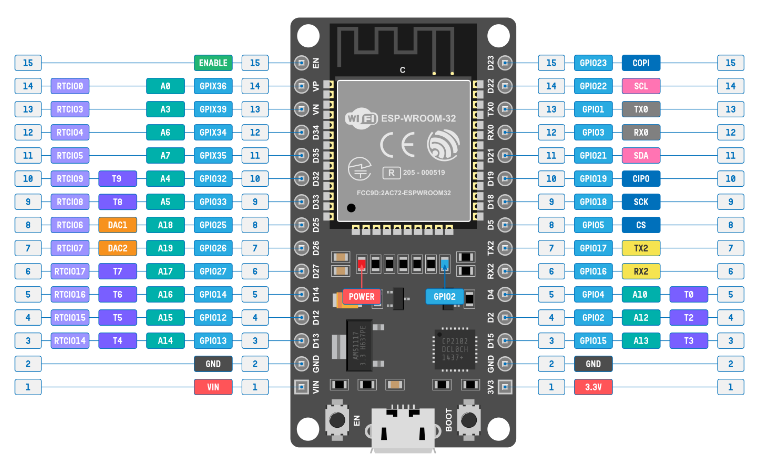
\includegraphics[width=13cm]{images/doit_devkit_v1.png}
   \caption{Schemat wyprowadzeń płytki DOIT DevKit V1 \cite{doitDevKitV1}}
   \label{Fig:devkitScheme}
\end{figure}

Jednym z kluczowych atutów platformy ESP32 jest wbudowane wsparcie dla Wi-Fi(802.11 b/g/n) i Bluetooth(klasyczny 4.2 i BLE), co umożliwia łatwe połączenie z siecią bezprzewodową oraz sprawną komunikację między urządzeniami zewnętrznymi.
Duża licz\-ba portów wejścia/wyjścia czyni go idealnym do obsługi wielu czujników, akscesoriów i modułów. Układ zawiera także zintegrowany konwerter analogowo-cyfrowy (ADC) umożliwiając precyzyjny pomiar sygnałów analogowych. System zawiera wiele innych możliwości, ale najważniejsze jego funkcjonalości i charakterystyczne cechy, firma Espressif zebrała na digramie,  który znalazł się na rysunku \ref*{Fig:functionalDiagram}.

\begin{figure}[ht]
   \centering
   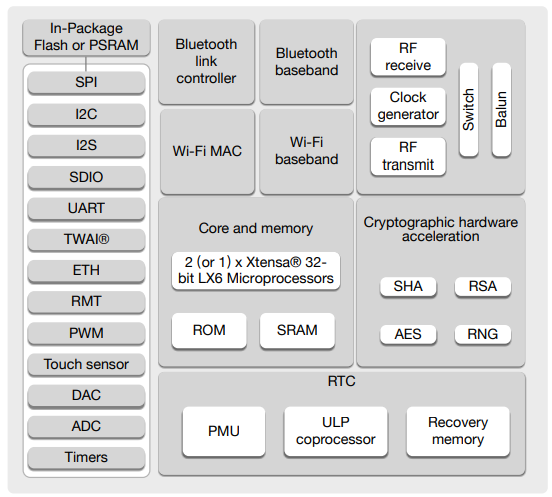
\includegraphics[width=12cm]{images/esp32_functional_diagram.png}
   \caption{Diagram funkcjonalności zaczerpnięty z dokumentacji techniczej ESP32\cite{esp32Datasheet}}
   \label{Fig:functionalDiagram}
\end{figure}

ESP32 został zoptymalizowany pod kątem efektywnego zużycia energii, co sprawia, że jest bardzo dobrym
wyborem dla aplikacji zasilanych bateryjnie lub kiedy ważny jest niski pobór prądu projektowanego systemu. Jego wszechstronność objawia
się obsługą przeróżnych protokołów komunikacji przewodowej,
takich jak SPI, I2C, UART, co sprawia, że integrację z zewnętrznymi modułami i systemami, można przeprowadzić w szybki i dostosowany do konkretnego przypadku sposób.

Warto podkreślić, że ESP32 cieszy się uznaniem wśród deweloperów, co przekłada się na dostęp do obszernej dokumentacji oraz wsparcie online na forach użytkowników. Programowalność w języku Arduino oraz możliwość korzystania
z MicroPython dodatkowo zwiększają elastyczność platformy, umożliwiając dostosowanie do indywidualnych potrzeb projektu.
Nieocenione są także biblioteki i moduły tworzone przez społeczność i udostępniane w formie otwartoźródłowej.
\subsection{Język programowania C++}
C++ jest językiem programowania, który swoje zastosowanie znalazł w wielu dziedzinach, gdzie ceni się wydajność rozwiązania. Mimo tego, że powstał w latach 80-dziesiątych na podstawie języka C, jego najnowsze wersje zdecydowanie można zaliczyć do nowoczesnych języków programowania.

Język ten jest kompilowany oraz stosuje silne typowanie statyczne, dzięki czemu, wykrywanie błędów na etapie tworzenia kodu jest znacznie łatwiejsze niż w przypadku innych podejść tworzenia programu wynikowego. Charakteryzuje się on także niskopoziomowym dostępem do pamięci, jak i możliwością jej dynamicznej alokacji w trakcie trwania programu, co zapewnia elastyczność implementacji i wysoką wydajność. C++ daje także możliwość korzystania z specyfikatora inline, który użyty dla funkcji powoduje, że kompilator kopiuje jej kod w zadane miejsce zamiast umieszczać tam wkaźnik do niej. Przekłada się to na minimalizację narzutu czasowego związanego z wywołaniami bloków funkcyjnych. Język ten umożliwia także stosowanie podejścia obiektowego do projektowania oprogramowania, co z kolei sprzyja modularności rozwiązania i łatwości utrzymania kodu.\cite{cppBjarne}

Wydajność i możliwość niskopoziomowej kotroli zasobów urządzenia powoduje, że język ten jest  najczęściej używany do programowania skomplikownych gier
komputerowych, protokołów komunikacyjnych oraz systemów wbudowanych. Przez jego popularność dla systemów osadzonych, powstało wiele współracujacych z nim frameworków i bibliotek do obsługi rozmaitych mikrokontrolerów. Dzięki temu wybierając C++ jako język tworzenia oprogramowania systemu wbudowanego zyskuje się bardzo dużą kontrolę nad sprzętem oraz elastyczność w doborze narzędzi deweloperskich.

\subsection{Framework Arduino}
Framework Arduino\cite{arduinoIntroduction} to otwarte oprogramowanie, które umożliwia łatwe tworzenie aplikacji dla mikrokontrolerów zgodnych z standardem płytek Arduino. Bazuje na języku programowania C++ oraz wykorzystuje uproszczoną warstwę abstrakcji, co sprawia, że jest przyjazny dla początkujących, jednocześnie oferując zaawansowane funkcje dla doświadczonych programistów.

Framework oferuje prostą obsługę wejścia/wyjścia (I/O), dzięki czemu integracja z czujnikami, przekaźnikami, i wieloma innymi modułami jest błyskawiczna i intuicyjna. Ponadto, zapewnia prosty sposób dostęp do interfejsów komunikacyjnych,
takich jak UART, SPI czy I2C. Ważną częścią frameworka Arduino są też przyjazne w użyciu biblioteki tworzone także przez użytkowników, przez co niemal zawsze znajdzie się kod obsługujący żądaną funkcjonalność. Obejmują one obszar komunikacji bezprzewodowej, obsługi czujników, sterowania silnikami, czy obsługi ekranów LCD i OLED. Każde z nich są regularnie poprawiane przez firmę lub społeczność dzięki czemu oprogramowanie staje się szybko aktualne i wspiera nowo dodane urządzenia i narzędzia.
\subsection{Komunikacja za pomocą podczerwieni}
Komunikacja przez podczerwień\cite{infrared} (IR - Infra-Red) to forma przesyłania danych, wykorzystująca fale elektromagnetyczne
o niższej częstotliwości niż światło widzialne. Fale podczerwone znajdują się w zakresie elektromagnetycznym
poniżej czerwonego końca widma światła widzialnego, typowo w zakresie od 300 GHz do 400 THz. Te fale są
niewidoczne dla ludzkiego oka, ale mogą być wykrywane i generowane przez diody. Typowo
wysyłając sygnał według konkretnego protokołu najpierw moduluje się go według określonego kodu liczbowego.
Modulacja może obejmować zmianę amplitudy, częstotliwości lub fazy fali podczerwonej. Gdy sygnał dociera do odbiornika
(zazwyczaj zasięg wynosi do 10m), odbiornik wyposażony także w diodę interpretuje odebrany sygnał, przeprowadzając proces demodulacji do kodu
liczbowego. Z tak wysłanej informacji może teraz skorzystać urządzenie odbierające i podjąć na jej podstawie działania.

W standardzie NEC\cite{necIR}, czyli najpopularniejszym sposobie przesyłania sygnałów do urządzeń RTV za pomocą światła podczerownego, zastosowana jest modulacja częstotliwośći. Każda wiadomość w tym typie komunikacji rozpoczyna się od stosunkowo długiego stanu wysokiego natężenia światła trwającego 9 ms, po czym następuje 4,5 ms przerwy sygnalizując tym samym rozpoczęcie nadawania. Chcąc teraz wysłać logiczną ,,1'' , należy wygenerować stan wysoki natężenia światła podczerwonego na 562.5µs i po nim odczekać 562.5µs nie wysyłając już niczego. Logiczne ,,0'' wysyłane jest przez taki sam zabieg, jednak z przerwą po stanie wysokim wynoszącą 1.6875 ms. Aby bit został odczytany przez odbiornik każda przerwa musi być zakończona następnym stanem wysokim natężenia fali światła, dlatego kiedy kończona jest transmisja, po ostatniej przerwie generowany jest dodatkowy puls długości 562.5µs, aby odbiornik mógł odczytać długość przerwy ostatniego bitu. Wykres ilustrujący elementarna generację sygnału w tym standardzie przedstawia rysunek \ref*{Fig:necOnesZerosFigure}.
\begin{figure}[ht]
   \centering
   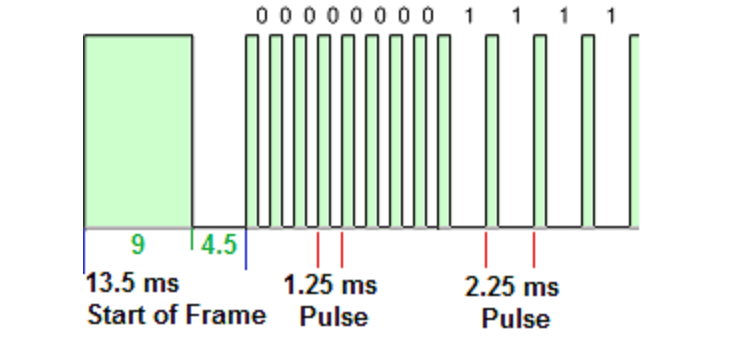
\includegraphics[width=8cm]{images/necOnesAndZeros.png}
   \caption{Wykres elementarnej modulacji sygnału standardu NEC}
   \label{Fig:necOnesZerosFigure}
\end{figure}

Aby wysłać pełne rządanie, które może być interpretowane przez odbiornik, trzeba wysłać informację opatrzoną w pewną strukturę. Najpierw wysyłany jest sygnał rozpoczęcia nadawania. Następnie wysyłany jest 8 bitowy adres urządzenia odbierającego sygnał i kolejno jego negacja bitowa. W takim sam sposób wysyłane jest 8 bitów danych i ich negacja bitowa. Tak zbudowana pojedyncza ramka danych, potrzebuje zawsze 67,5 ms, aby zostać wysłaną, niezależnie od wysyłanych danych i adresu urządzenia dzięki negacji bitowej obu tych segmentów. Przykładowe wysłanie kodu liczbowego 0xAD do urządzenia o adresie 0xFF przedstawione zostało na wykresie znajdującym się na Rys.\ref*{Fig:necFrame}.

\begin{figure}[ht]
   \centering
   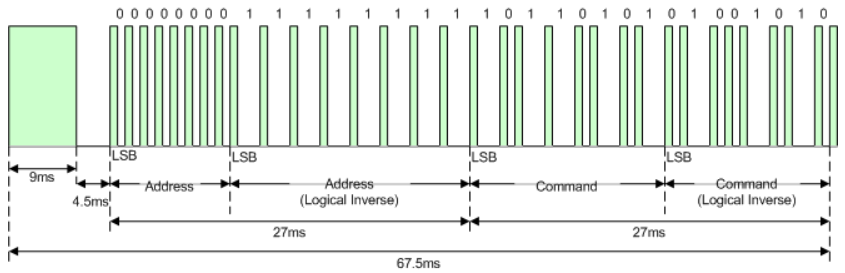
\includegraphics[width=13cm]{images/necFrame.png}
   \caption{Przykładowa modulacja sygnału pełnej wiadomości standardu NEC}
   \label{Fig:necFrame}
\end{figure}

\subsection{System operacyjny Android}
System Android, rozwijany przez firmę Google, stanowi środowisko operacyjne oparte na otwartym kodzie źródłowym. Przyczynia się to do jego wyjątkowej elastyczności i dostosowywalności do różnych urządzeń mobilnych, głównie
smartfonów i tabletów, ale z powodzeniem stosowany jest także w innych urządzeniach przenośnych.

Otwartość kodu umożliwia deweloperom z całego świata dostosowywanie systemu do specyficznych potrzeb. Istotną cechą Androida jest także jego wszechstronność, manifestująca się w szerokiej gamie dostępnych
urządzeń pracujących z tym systemem operacyjnym.
Instalowany jest on na urządzeniach z wszystkich przedziałów cenowych, umożliwiając
programistom tworzenie aplikacji dostępnych dla każdej z grup odbiorców. Sklep Google Play, jako główne źródło
aplikacji, gier, multimediów i innych treści, stanowi istotny element ekosystemu Androida. Ponadto, integracja
z usługami Google, takimi jak Gmail, Google Drive, Google Maps i wielu innych sprawia, że można niemal każdą czynność wykonać przy pomocy dedykowanej aplikacji firmy Google. Względna jednolitość tego środowiska, pomimo takiej gamy obsługiwanych urządzeń sprawia, że dla programistów stanowi ono atrakcyjne pole do
rozwoju i tworzenia innowacyjnych rozwiązań. Platforma jest też bradzo opłacalnym polem biznesowym z uwagi na szeroką bazę użytkowników oraz dynamiczny rynek aplikacji mobilnych. Nie jest więc dziwne, że urządzenia z Androidem posiadało 69,74\% wszytskich użytkowników urzadzeń mobilnych i był on wciąż najczęściej używanym systemem operacyjnym w 2022 roku\cite{androidStats}.
\subsection{Język programowania Dart}
Dart to język programowania stworzony przez Google, zaprojektowany z myślą o tworzeniu wydajnych, skalowalnych i nowoczesnych aplikacji. Jego głównym zastosowaniem jest budowa interaktywnych stron internetowych oraz aplikacji mobilnych przy użyciu zestawu narządzi Flutter.

Język ten charakteryzuje się statycznym typowaniem, co oznacza, że typy zmiennych sprawdzane są w trakcie budowania aplikacji, co może pomóc w wykrywaniu błędów przed uruchomieniem programu. Dart wspiera i opiera się głównie na programowaniu obiektowym.

Jedną z ważnych cech Darta, jest również jego zdolność do wykonywania kodu zarówno w trybie just-in-time (JIT) jak i ahead-of-time (AOT). Tryb JIT umożliwia szybkie rozwijanie i testowanie aplikacji, podczas gdy tryb AOT pozwala na kompilację
kodu źródłowego do natywnego kodu maszynowego, co zwiększa wydajność aplikacji podczas działania. Dart oferuje także mechanizmy asynchroniczne, co jest niezwykle istotne w programowaniu współbieżnym i obsłudze operacji wejścia/wyjścia bez blokowania głównego wątku.\cite{dartInfo}

W kontekście frameworka Flutter, język ten staje się kluczowym narzędziem budowy interfejsów użytkownika. Sam wspomniany zestaw narzędzi został napisany przy pomocy Darta i to z nim najlepiej współpracuje.
\subsection{Framework Flutter}
Flutter to otwartoźródłowy zestaw narzędzi (SDK - Software Development Kit) stworzony przez Google do budowy interfejsów użytkownika (UI - User Inferface). Jest wykorzystywany do tworzenia aplikacji mobilnych, webowych i desktopowych, ze wskazaniem na aplikacje mobilne. Jednym z głównych atutów Fluttera jest możliwość tworzenia jednego kodu źródłowego, który może być budowany do aplikacji dla różnych platform, takich jak Android, iOS, web, Windows czy Linux.

W centrum Fluttera znajduje się Dart, który jest używany do definiowania interfejsu użytkownika oraz logiki biznesowej.
SDK ten bazuje na podejściu deklaratywnym, co oznacza, że w kodzie opisuje się, jak ma wyglądać interfejs w danym momencie, a nie, jak ma być aktualizowany w odpowiedzi na różne zdarzenia. To podejście ułatwia zrozumienie i utrzymanie kodu.
Wprowadza on również własny silnik renderujący. Dzięki temu, dobrze zaprojektowane aplikacje Fluttera charakteryzują się płynnością i responsywnością.

Zestaw oferuje bogatą gamę wbudowanych widgetów, które są podstawowymi elementami budującymi interfejs użytkownika. Programiści mogą również tworzyć własne niestandardowe widgety, co umożliwia pełną swobodę w projektowaniu UI.

Flutter wspiera hot-reloading, co pozwala na natychmiastowe obserwowanie zmian wprowadzanych w kodzie bez konieczności ponownego uruchamiania całej aplikacji. Korzystanie z tego mechanizmu znacznie skraca się czas pracy podczas rozwijania projektu.
Dzięki narzędziom takim jak Flutter DevTools, umożliwiony jest dostęp do zaawansowanych narzędzi do analizy, debugowania i optymalizacji aplikacji końcowej.\cite{flutterDocs}

Framework ten stał się niebywale popularny wśród programistów. Chcąc tworzyć estetyczne, responsywne i wieloplatformowe aplikacje z minimalnym nakładem pracy, mając do dyspozycji obszerną i interaktywną dokumnetację, jednym z najlepszych wyborów jest wybranie Fluttera jako główne nardzędzie tworzenia interfejsu użytkownika.
\subsection{Komunikacja przez Bluetooth Low Energy}
Bluetooth Low Energy(BLE)\cite{ble} to technologia komunikacyjna zaprojektowana do efektywnej wymiany danych pomiędzy urządzeniami przy niskim zużyciu energii. Jest uproszczoną i zoptymalizowaną wersją klasycznego Bluetooth.
Komunikacja za pomocą BLE opiera się na koncepcji dwóch głównych typów urządzeń: urządzenia peryferyjnego i centralnego. Urządzenie peryferyjne emituje dane, podczas gdy urządzenie centralne zbiera te dane.

Cechą charakterystyczną BLE jest niskie zużycie energii, co sprawia, że jest idealny do zastosowań, gdzie ważne jest przedłużenie życia baterii w urządzeniach przenośnych. Komunikacja BLE opiera się na transmisji krótkich pakietów danych, co przyczynia się do wysokiej efektywności energetycznej.

Usługi w BLE to logiczne grupy charakterystyk, które reprezentowane są jako zestawy danych, udostępniające funkcjonalności lub zestawy operacji odpowiednie dla danej grupy. Charakterystyki z kolei to konkretne funkcje lub dane w ramach danej usługi. GATT (Generic Attribute Profile) jest z kolei protokołem używanym w BLE do opisu i komunikacji z usługami i charakterystykami poprzez klienta GATT. Każda usługa i charakterystyka posiada swój numer UUID.

Komunikacja między urządzeniem centralnym, a peryferyjnym, opiera się na zestawie reguł znanych jako GATT Server (na urządzeniu peryferyjnym) i GATT Client (na urządzeniu centralnym). GATT Server udostępnia usługi i charakterystyki, natomiast GATT Client korzysta z protokołu GATT do odczytywania i zapisywania danych.

Wiele bibliotek na rożne platformy sprzętowe umożliwia łatwe i szybkie obsługiwianie technologii Bluetooth Low Energy przez wydzielenie na wysokim poziomie abstrakcji funkcji, obiektów i metod zdecydowanie ułatwiających korzystanie z tej technologii. Takie podejście zwalnia z programisty obowiązek zajęcia się niuansami w projektach, w których nie są one krytycznymi elementami rozwiązania i pozwala na uniknięcie trudnych do zdiagnozowania błędów konfiguracji.

\clearpage

\section{Urządzenie wysyłające sygnały IR}
\subsection{Schemat elektryczny zaprojektowanego urządzenia}
Aby wykonać urzadzenie pośredniczące najpierw wykonano shemat elektryczny przy pomocy programu EasyEDA w darmowej wersji online\cite{easyEda}. Dzięki bibliotekom tworzonym przez użytkowników odnaleziono wszystkie niezbędne elementy do działania urządzenia pośredniczącego. Utworzony schemat elektryczny powstały z użytych komponentów znajduje się na Rys. \ref*{Fig:deviceScheme}.
\begin{figure}[ht]
   \centering
   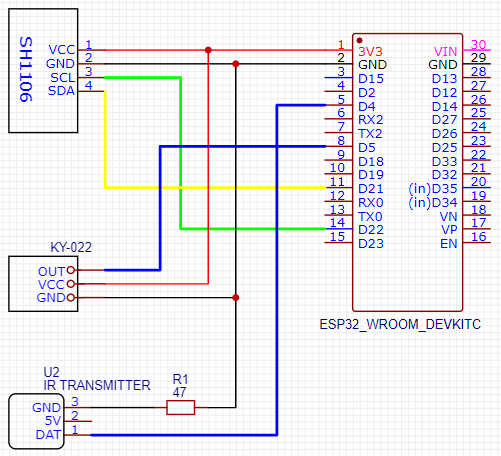
\includegraphics[width=12cm]{images/deviceScheme.png}
   \caption{Schemat elektryczny urządzenia pośredniczącego}
   \label{Fig:deviceScheme}
\end{figure}

Na schemacie kolorem czarnym oznaczono połączenia do masy (GND), kolorem czerwonym zasilanie z mikrokontrolera o potencjale 3.3V. Na niebiesko zaznaczone są szyny danych modułów IR. Z kolei kolorem zielonym oznaczono linię zegarową, a żółtym linię danych,porotokołu komunikacjynego I2C wyświetlacza OLED.

Samo urządznie nie jest wrażliwe na zakłócenia elektromagnetyczne, ani nie wymagało ochronnej obudowy do przestestowania poprawności założeń projektowych oraz końcowych testów pełnego systemu, dlatego jako element łączący moduły została użyta płytka stykowa. Dzięki użyciu płytki zachowano pełną funkcjonalność urządzenia oraz zyskano dowolność zmian podczas projektowania rozmieszczenia i połączenia komponentów. Urządznie osadzone na płytce prototypowej zostało przedstawione na Rys. \ref*{Fig:deviceOnBoard}.
\begin{figure}[ht]
   \centering
   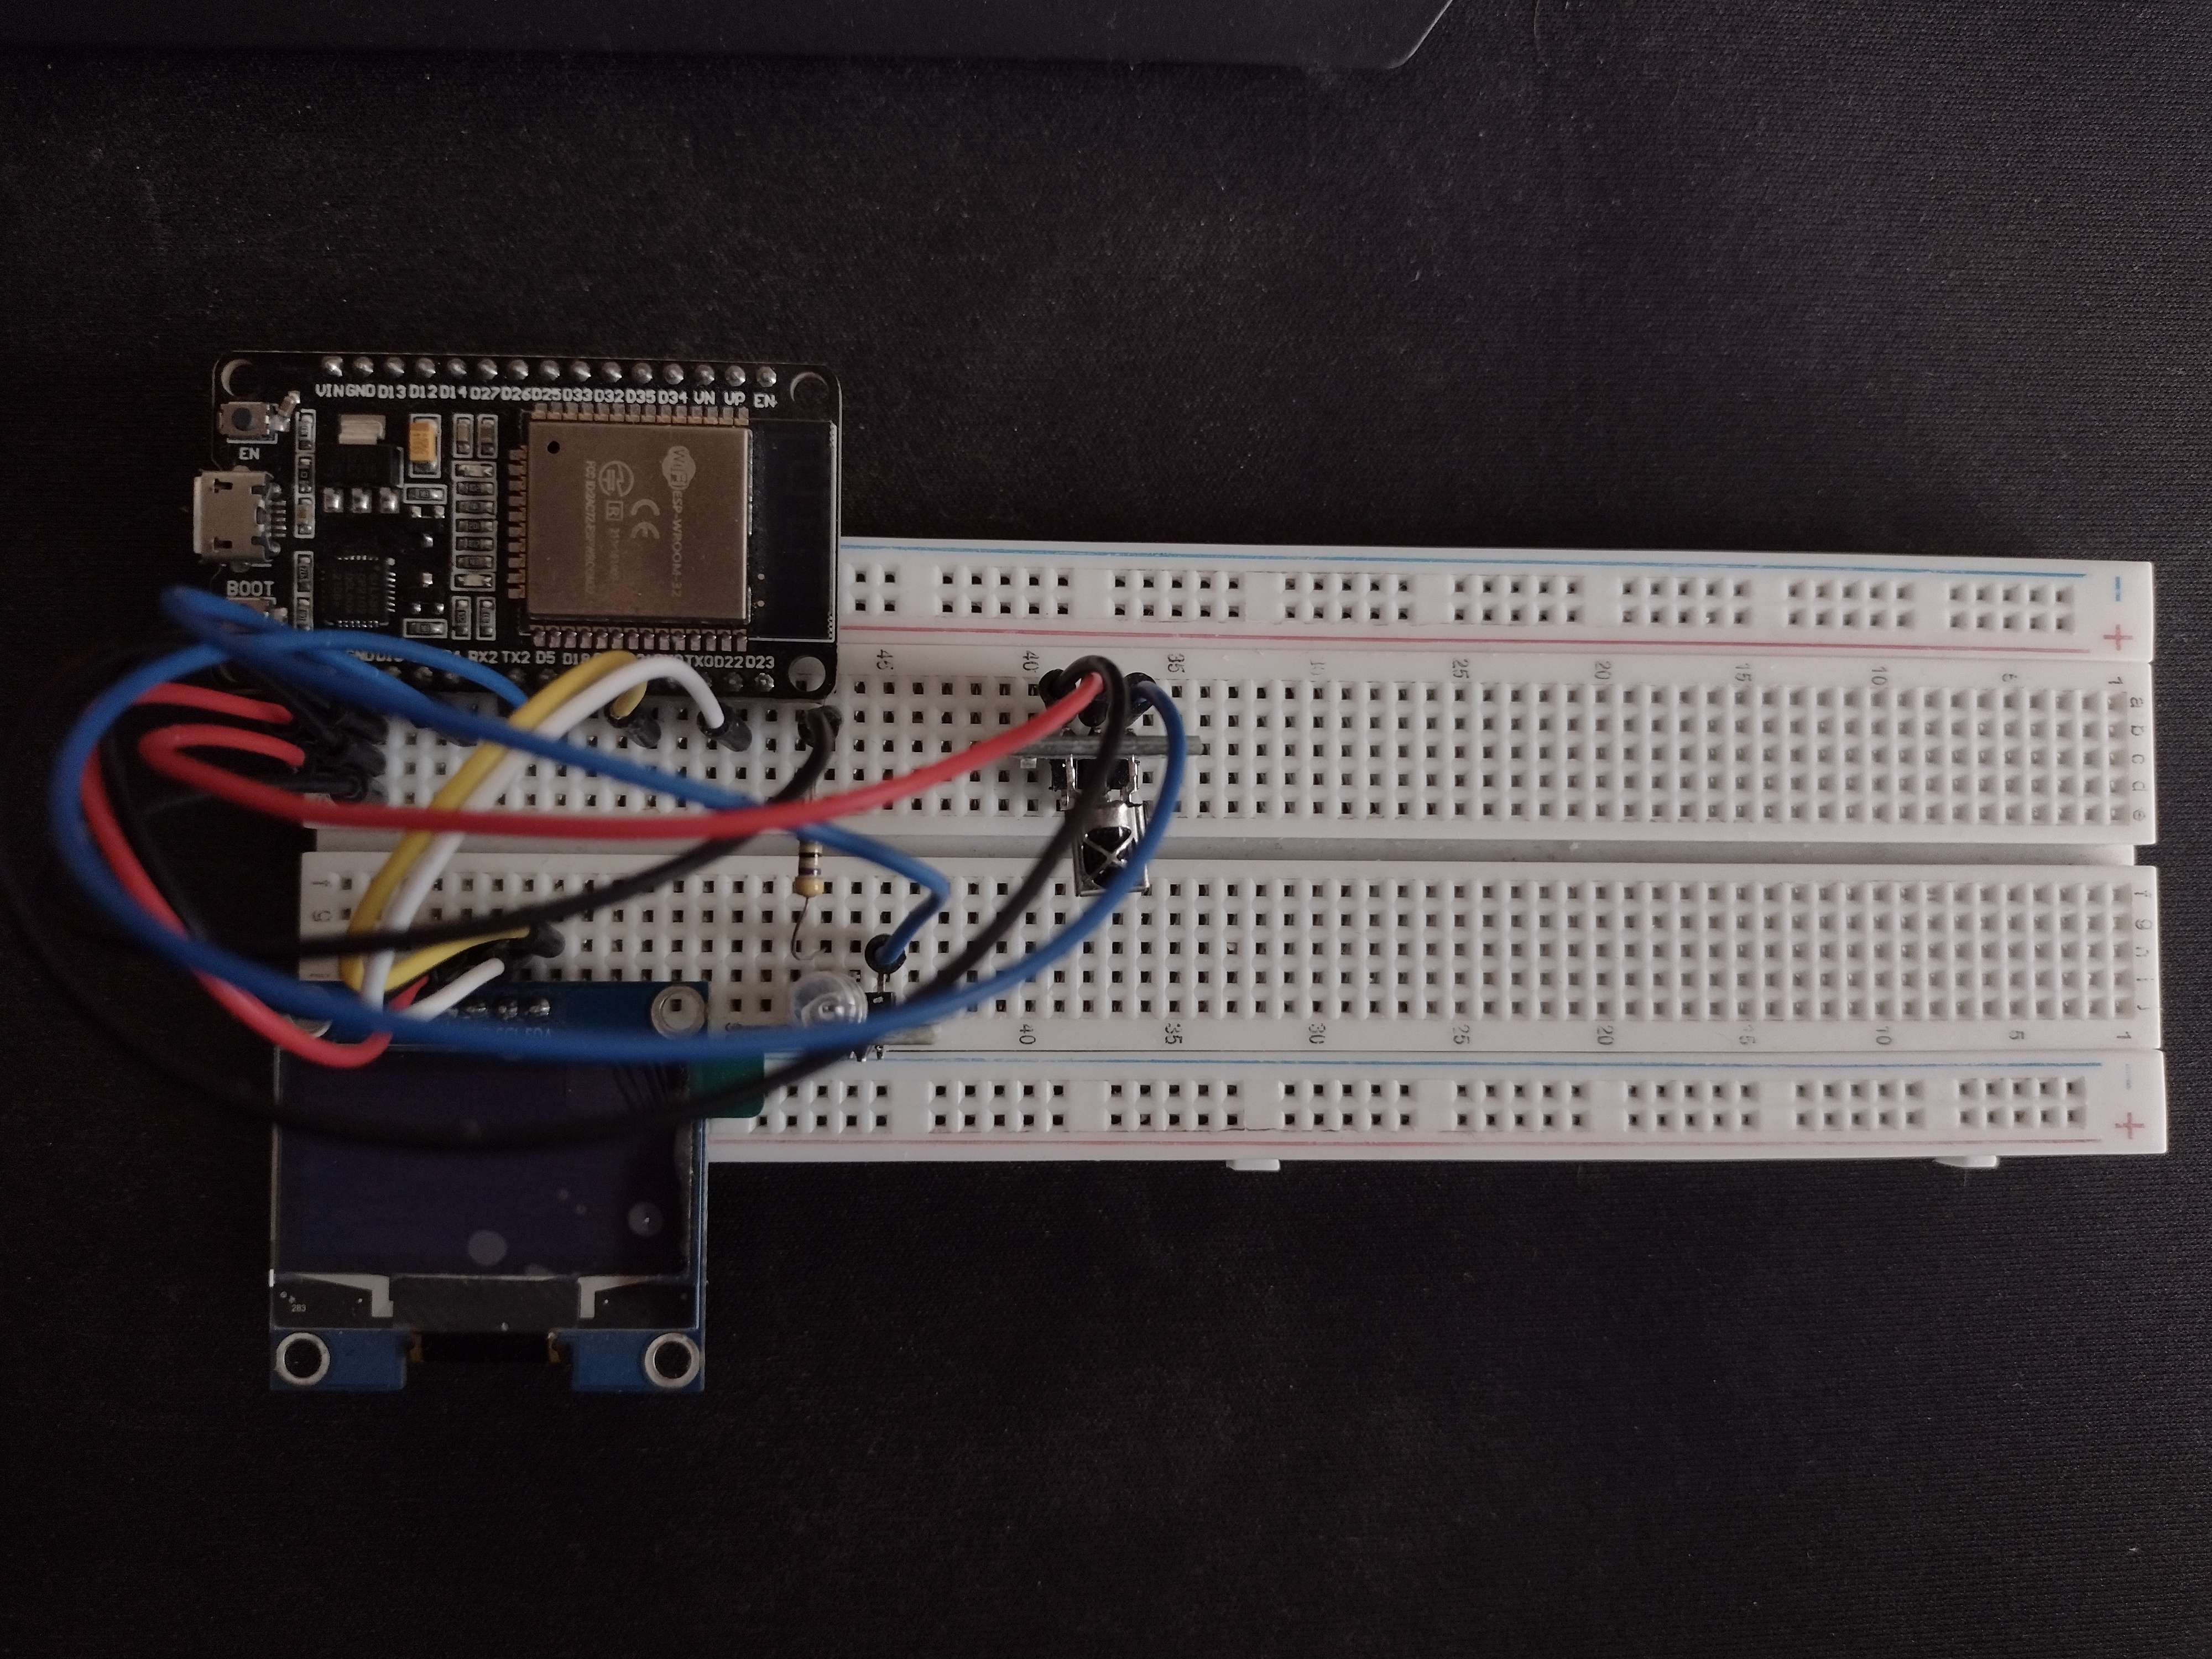
\includegraphics[width=12cm]{images/deviceOnBoard.jpg}
   \caption{Urządzenie pośredniczące osadzone na płytce prototypowej}
   \label{Fig:deviceOnBoard}
\end{figure}
\subsection{Przegląd i opis użytych komponentów}
Elementy przedstawione na schemacie elektrycznym znalazły się w przedstawionym wcześniej modelu modelu fizycznym. Są to:
\begin{enumerate}[label=\alph*), leftmargin=1.25cm]
   \item Płytka deweloperska ESP32 Wroom DevKitC V1\cite{doitDevKitV1} - to system z mikrokontroler ESP32 z procesorem Dual Core Tensilica LX6 240 MHz, pamięcią SRAM 520 KB i pamięcią flash 4 MB. Posiada wbudowane moduły WiFi 802.11 b/g/n oraz moduł Bluetooth Low Energy, dzięki którym nie trzeba dołączać osobnych modułów komunikacji bezprzewodowej. Znajduje się na nim 30 wyprowadzeń GPIO w postaci goldpinów, co znacznie zwiększa wygodę projektowania. Zasilany jest z 5 V ze złącza microUSB lub pinu VCC i GND.
   \item Wyświetlacz OLED SH1106\cite{sh1106}- to wyświetlacz OLED o przekątnej 1,3'' i rozdzielczości 128 pikseli na 64 pikesle. Ekran oparty jest na sterowniku Adafruit SH1106 pracuje z napięciami 3,3 V oraz 5 V, komunikuje się poprzez protokół I2C. Posiada wlutowane proste złącza goldpin. Wyświetla znaki w kolorze białym.
   \item Transmiter IR KY-005\cite{ky005} - to moduł nadawczy sygnałów podczerownych. Obsługuje wysyłanie fal IR o długości 940nm. I pobiera 90mW mocy podczas działania.
   \item Odbiornik IR KY-022\cite{ky022}  - to moduł z odbiorczy podczerwieni, działający na częstotliwości 38 kHz. Zasilany jest napięciem od 2,7 V do 5,5 V. Wykrywa sygnał pod maksymalnym kątem odchylenia 90°. Maksymalna odległość wykrywania: 18 m. Posiada cyfrowy sygnał wyjściowy.
   \item Rezystor 47 Ohm - resystor przewlekany o tolerancji 5\% i makasymalnej mocy 0,25 W.
   \item Przewody połaczeniowe męsko-męskie.
   \item Płytka stykowa.
\end{enumerate}

\clearpage

\section{Oprogramowanie sterujące urządzeniem wysyłającym sygnały IR}
\subsection{Środowisko narzędziowe}
Kod sterujący urządzeniem pośredniczącym opartym o mikrokontroler ESP32 został przygotowany za pomocą jezyka C++ oraz frameworka Arduino. Cały projekt oprogramowania zarządzany był przez rozszerzenie do edytora tekstu Visual Studio Code, czyli PlatformIO, przy pomocy którego były doinstalowywane też wymagane biblioteki oraz budowany i wgrywany na płytkę ESP32 Wroom DevKitC był program sterujący, a także przeprowadzane debugowanie. Każda z tych operacji mogła się odbyć dzięki wsparciu programowania i debugowania za pomocą portu microUSB, które posiadała płytka oraz rozszerzenie edytora tekstu.
\subsection{Ogólna struktura oprogramowania}
Oprogramowanie sterujące urządzeniem wysyłąjącym sygnały podczerowne zostało podzielone na 4 elementy. Główny z nich to plik main.cpp gdzie odbywa się sterowanie urządzeniem, korzystając przy tym z pozostałych modułów. Utworzone zostały 3 moduły narzędziowe, aby główny kod stał się bardziej przejrzysty oraz modularny. Opdowiadają one za obsługę wyświetlacza OLED, komunikację BLE oraz interpretację danych pochodzących z charakterystyk BLE. Wynikowa struktura podziału autorskich elementów oprogramowania została przedstawiona na Rys. \ref*{Fig:codeStructure}.
\begin{figure}[ht]
   \centering
   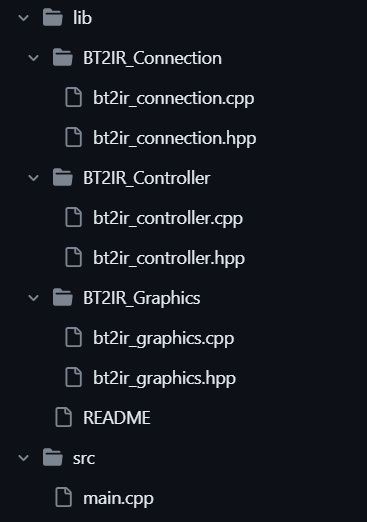
\includegraphics[width=4.5cm]{images/codeStructure.png}
   \caption{Struktura oprogramowania sterującego urządzeniem pośredniczącym}
   \label{Fig:codeStructure}
\end{figure}

\subsection{Główny program sterujący}
Główny program, który steruje urządzeniem pośredniczącym znajduje się w pliku ,,main.cpp''. Aby zorzumieć jakie funkcjonalności oferuje, najlepiej prześledzić jego budowę.

Najpierw dołączane są pliki nagłówkowe z frameworka Arduino dla ESP32 odpowiadające za obsługę wysyłu i odbioru syngałów podczerwonych. Dołączane są także autorskie moduły z przestrzeni nazw ,,bt2ir''. Korzystając z nich z kolei można utworzyć globalne obiekty klas, które pozwalają na zarządzanie połączeniem BLE, interpretację danych z charakterystyk tego połączenia, i pracę z  wyświetlaczem OLED. Obiekty tych klas zostają zinicjowane odpowiednimi danymi, prawidłowymi dla posiadanego sprzętu, jak rozdzielczość ekranu OLED czy numery pinów płytki deweloperskiej, na których będą przesyłane dane z i do modułów IR. Kod realizujący dołączanie plików nagłówkowych oraz inicjalizację obiektów globalnych znajduje się na List. \ref{Lst:globalDefinitions}.

\lstinputlisting[inputencoding=utf8/cp1250, language={C++}, caption={\protect\input{captions/globalDefinitions.txt}\protect\relax}, label={Lst:globalDefinitions}]{codes/globalDefinitions.cpp}

Framework Arduino oczekuje zedefiniowania funkcji ,,setup()'', która będzie wykonywana raz podczas uruchomienia urządzenia. Utworzono takową i zawarto w niej już na początku zainicjowanie połaczenia szeregowego, aby móc odczytywać dane z urządzenia, na wypadek chęci wykrycia błędów działania. Znalazła się tam także inicjacja połaczenia z wyświetlaczem OLED poprzez protokół I2C oraz inicjacja serwera BLE, obie inicjacje zostały przeprowadzone za pomocą metod obiektów klas z autorskich modułów. Rozpoczęto w tej funkcji już nasłuchiwanie sygnałów podczerwonych i zainicjowano pracę modułu wysyłającego sygnały IR przy pomocy wcześniej utworzonych obiektów. Zawartość funkcji ,,setup()'' przedstawia kod źródłówy na listingu List.\ref*{Lst:setup}.

\lstinputlisting[inputencoding=utf8/cp1250, language={C++}, caption={\protect\input{captions/setup.txt}\protect\relax}, label={Lst:setup}]{codes/setup.cpp}

Tworząc oprogramowanie za pomocą frameworka Arduino zdefiniować należy także funkcję, która będzie wykonywana w nieskończonej pętli na programowanym urządzeniu. Narzędzie wymaga nazywała się ona ,,loop()''. Przed nią jednak znalazły się jeszcze inicjalizacje dwóch znaczników czasowych w postaci dodatnich liczb całkowitych, które zostaną użyte do odliczania czasu trwania wyświetlania komunikatów dla użytkownika.

W samej już funkcji umieszczono instrukcje warunkowe, przez które, sprawdzane jest czy wstąpiły zdarzenia, takie jak: odebranie danych za pomocą serwera BLE o wciśniętym klawiszu w aplikacji, odebranie sygnału podczerwonego na module odbiornika IR, czy też rozłączenie lub połączenie z serwerem BLE nowego użytkownika aplikacji mobilnej. Jeśli program wykryje zdarzenie serwera BLE, rysuje na wyświetlaczu OLED odświeżony stan połaczenia zwierający informację o liczbie połączonych użytkowników. Jeśli z kolei wykryte zostanie zdarzenie odebrania na serwerze BLE informacji o typie wciśniętego przycisku, rysowana jest jego ikona i nazwa, aby poinformować użytkownika o otrzymaniu jego żądania. Po obsłużeniu zdarzenia resetowana jest flaga informująca o jego aktywności. Obsługa opisanych zdarzeń w pierwszej części funkcji ,,loop()'' została przedstawiona na List. \ref*{Lst:loop1}.
\lstinputlisting[inputencoding=utf8/cp1250, language={C++}, caption={\protect\input{captions/loop1.txt}\protect\relax}, label={Lst:loop1}]{codes/loop1.cpp}

Program reaguje też na otrzymanie szesnastkowego kodu IR po wciśnieciu przycisku  pilota w aplikacji mobilnej. Po otrzymaniu tego kodu przez BLE, przesyłany jest on dalej w formie sygnału podczerwonego do telewizora, realizując w ten sposób sterowanie nim, po zakończeniu już obsługi zdarzenia resetowana jest jego flaga. Jeżeli odczytany zostanie na zewnętrznym module odbiorczym, prawidłowy sygnał podczerwony, wypisany zostaje on na wyświetlaczu OLED, dzięki dedykowanej metodzie obiektu sterującego tym ekranem. Aktualizowany zostaje też wtedy znacznik czasowy tego zdarzenia. Następnie też wznawiane jest nasłuchiwanie sygnałów podczerwonych. Każdy z komunikatów dla użytkownika posiada swój czas wyświetlania. Limitowanie czasu ich trwania jest realizowane za pomocą sprawdzania stempli czasowych. Jeśli któryś z komunikatów powinien już się zakończyć, co jest wnioskowane na podstawie odległości aktualnego czasu od odpowiedniego znacznika czasowego, resetowane są wszystkie znaczniki czasowe komunikatów i następuje wyświetlenie domyślnego ekranu stanu połączenia BLE. Te funkcjonalności znalazły się w drugiej części funkcji ,,loop()'', a jej kod źródłowy został przedstawiony na List. \ref{Lst:loop2}.
\lstinputlisting[inputencoding=utf8/cp1250, language={C++}, caption={\protect\input{captions/loop2.txt}\protect\relax}, label={Lst:loop2}]{codes/loop2.cpp}
\subsection{Moduł komunikacji przez BLE}
Autorski moduł odpowiedzialny za komunikację BLE został oparty o moduły biblioteki NimBLE\cite{nimBLE}, zamiast podstawowej biblioteki przygotowanej przez Arduino, ponieważ ta druga zajmowała zbyt wiele miejsca i nie mieściła się w pamięci FLASH mikrokontrolera. Wszystkie elementy tego modułu znalazły się w przestrzeni nazw ,,bt2ir''.

Klasa zarządzająca połaczeniem BLE została utworzona przy pomocy wzorca projektowego Singleton\cite{designPatterns}, który powoduje że użytkownich korzysta z logicznie tylko jednej instancji takiej klasy, przechowywanej pomiędzy obiektami za pomocą uchywtu, którym dla języka C++ stał się wskaźnik. Zasosowano ten wzorzec aby zachowywać informacje o połączeniu BLE w całym programie i modduły mogły korzystać jednocześnie z tego samego połącznia w wygodny sposób. Publiczne funkcjonalności tej klasy udostępnione za pomocą metod to:
\begin{enumerate}[label=\alph*), leftmargin=1.25cm]
   \item inicjalizacja serwera BLE
   \item możliwość odczytywania i edytowania liczby połączonych urządzeń
   \item możliwość odczytywania i edytowania flag zdarzeń odebrania danych wciśniętego przycisku w aplikacji mobilnej
   \item dostęp do charakterystyk odebranego typu przycisku i jego kodu IR
   \item metoda pozwalająca narysować aktualny stan połączenia BLE.
\end{enumerate} Część pliku nagłówkowego zawierająca dostępne metody publiczne klasy Connection została przedstawiona na List. \ref*{Lst:bleMethods}.

\lstinputlisting[inputencoding=utf8/cp1250, language={C++}, caption={\protect\input{captions/bleMethods.txt}\protect\relax}, label={Lst:bleMethods}]{codes/bleMethods.cpp}

Najważniejszym elementem tego modułu jest metoda setupConnection() klasy Connection. W niej właśnie odbywa się inicjowanie serwera BLE wraz z jego parametrami oraz dołączenie funkcji wywoływanych podczas zdarzeń serwera.

Podczas przygotowywania urządzenia pośredniczącego do obsługi BLE w pierwszej kolejności inicjowane jest abstrakcja urządzenia. Kolejno dalej na urządzeniu tworzony jest serwer i przypisywane są mu autorskie klasy przechowujące metody wywoływane przez zdarzenia serwera, zawarte także w tym module, dzięki czemu biblioteka automatycznie będzie wykonywać czynności po połączeniu i rozłączeniu użytkownika, oraz o takim wydarzeniu zostanie poinformowany główny program sterujący.
Na tak utworzonym serwerze tworzony jest serwis i jego 2 charakterystyki odpowiadające wyłącznie za odbieranie danych o typie wciśniętego przycisku i jego szesnastkowym kodzie IR. Obie charakterystyki otrzymują także swoje klasy z metodami wywoływanymi podczas odebrania danych, dzięki czemu główny program sterujący informowany jest o tym zdarzeniu. Utworzony w ten sposób serwer może rozpocząć rozgłaszanie swojej obecności i nazwiązywać połączenia z klientami. Kod funkcji realizującej inicjalizację serwera BLE znajduje się na List. \ref*{Lst:setupConnection}.

\lstinputlisting[inputencoding=utf8/cp1250, language={C++}, caption={\protect\input{captions/setupConnection.txt}\protect\relax}, label={Lst:setupConnection}]{codes/setupConnection.cpp}

Aby uzyskać możliwość połaczenia wielu użytkowników z serwerem BLE urządzenia pośredniczącego metoda wywoływana podczas każdego połączenia nowego użytkownika musi wznowić rozgłaszanie dostępności serwera. Ta funkcjonalność została zaimplementowana w funkcjach wywwoływanych podczas zdarzeń serwera.
\subsection{Moduł interpretujący dane z BLE}
Aby ułatwić pracę z danymi odebranymi przez urządznie pośredniczące utworzono moduł przetwarzający je. Zawiera on wygodny typ wylieczniowy wykorzystywany do nadawania przejrzystych nazw programowych dla odebranych typów wciśniętego przycisku pilota z aplikacji mobilnej.
Z kolei klasa Controller odpowiada za interpretację danych, odebranych za pomocą charakterystyk serwera BLE. Korzysta ona z instancji klasy Connection aby pobrać dane z charakterystyk i je przetworzyć. W tym celu, klasa ta, udostępnia metody pozwalające odświeżać przechowywane jej polach prywatnych ostatnio odebrane dane od aplikacji mobilnej. Publicznie dostępne elementy modułu znajdują się na List. \ref*{Lst:controller}.

\lstinputlisting[inputencoding=utf8/cp1250, language={C++}, caption={\protect\input{captions/controller.txt}\protect\relax}, label={Lst:controller}]{codes/controller.cpp}

Dane odebrane za pomocą charakterystyk przechowywane są w postaci bitowej. Aby odczytać ich wartości należy zinterpretować ich zawartość za pomocą odpowiedniego szablonu, który w tym przypadku będzie typem danych. Metoda updateButtonType() z klasy Controller interpretuje dane charakterystki za pomocą typu 8 bitowej liczby całkowitej bez znaku, ponieważ ilość przycisków jest niewielka. Odbywa się tam też prosta kontrola poprawności danych, poprzez sprawdzenie czy odebrane dane mieszczą się w zakresie zdefiniowanych przycisków pilota. Kod źródłowy tej funkcji znajduje się na List. \ref*{Lst:dataProcessing}.

\lstinputlisting[inputencoding=utf8/cp1250, language={C++}, caption={\protect\input{captions/dataProcessing.txt}\protect\relax}, label={Lst:dataProcessing}]{codes/dataProcessing.cpp}

\subsection{Moduł obsługi ekranu OLED}
Autorski moduł obsługi ekranu OLED jest w rzeczywistości nakładką na klasę sterującą wyświetlaczem OLED z bibliotek firmy Adafruit. Taka relacja realizowania jest za pomocą dziedziczenia publicznego po klasie ,,Adafruit\_SH1106G'' w utworzonej klasie nakładki ,,Display''. Sama nakładka znalazła się w przestrzeni nazw bt2ir.

Utworzona klasa nakładki stara się udostępnić metody, dzięki którym użytkownik w prosty i przejrzysty sposób może rysować konkretne obrazy i napisy na wyświetlaczu, w postaci przygotowanych i zparametryzowanych ekranów. Udostępnione zostały ekrany takie jak przedstawienie liczby połączonych smartfonów z serwerem BLE i jego stanu, wyświetlanie komunikatu o odebraniu wciśniętego przycisku z aplikacji mobilnej, czy wyświetlenia odebranego za pomocą modułu odbiorczego z diodą sygnału IR. Lista dostępnych funkcjonalności utworzonej nakładki w postaci metod publicznych została przedstawiona na List. \ref*{Lst:graphics}.

\lstinputlisting[inputencoding=utf8/cp1250, language={C++}, caption={\protect\input{captions/graphics.txt}\protect\relax}, label={Lst:graphics}]{codes/graphics.cpp}

Ukryta dla użtykownika logika tej nakładki opiera się o 4 metody prywatne. Dwie z nich rysują bardziej podstawowe elementy ekranów, takie jak rysowanie wyrównanego tekstu czy wielkich cyfr. Dzięki nim powstały także dwie metody z nich korzystające, przy pomocy których, można narysować na wyświetlaczu ikonę z podpisem lub cyfrę z podpisem. Tak wydzielone fragmenty logiki kodu, przyspieszyły i ułatwiły zbudowanie wszystkich publicznie dostępnych funkcjonalności. Utworzona lista prywatnych metod zaprojektowanej klasy znajduje się na List. \ref*{Lst:graphicsPrivate}.

\lstinputlisting[inputencoding=utf8/cp1250, language={C++}, caption={\protect\input{captions/graphicsPrivate.txt}\protect\relax}, label={Lst:graphicsPrivate}]{codes/graphicsPrivate.cpp}

Ikony rysowane na ekranach przez publiczne metody nakładki zostały umieszczone w programie za pomocą tablic bajtów, a same tablice zostały wygenerowane poprzez progowanie binarne obrazów w odcieniach szarości, przy pomocy aplikacji internetowej image2cpp[]. Po przekonwertowaniu obrazów na tablice bajtów i usunięciu z jej otoczenia niepotrzebnie wygenerowanych części kodu, można ją umieścić w oprogramowaniu i wykorzystywać do wyświetlania obrazu, którego ta tablica dotyczy. Jedna z wygenerowanych tablic znajduje się na List. \ref*{Lst:imageArray}.

\lstinputlisting[inputencoding=utf8/cp1250, language={C++}, caption={\protect\input{captions/imageArray.txt}\protect\relax}, label={Lst:imageArray}]{codes/imageArray.cpp}

Dzięki utworzonym narzędziom budowano publiczne metody dostępne dla użytkownika nakładki. W każdej takiej funkcji najpierw czyszczony był wyświetlacz, następnie rysowano w buforze ekranu odpowiedni obraz na podstawie zdefiniowanych tablic bajtów wraz z wyśrodkowanym podpisem, by końcowo wyświetlić dane zgromadzone w buforze rysowania. Jedną z tych metod jest ,,drawMoveUp()'' rysująca komunikat dla użytkownika o wciśnięciu przycisku przejścia w górę na pilocie w aplikacji mobilnej. Jej implementacja została przedstawiona na List. \ref*{Lst:drawMoveUp}, a jej fizyczny efekt na wyświetlaczu OLED pokazano na Rys. \ref*{Fig:drawMoveUp}.

\lstinputlisting[inputencoding=utf8/cp1250, language={C++}, caption={\protect\input{captions/drawMoveUp.txt}\protect\relax}, label={Lst:drawMoveUp}]{codes/drawMoveUp.cpp}

Więcej ekranów i obrazów, które może też przedstawiać wyświetlacz OLED osadzony w urządzeniu pośredniczącym zostały zawarte w prezentacji pełnego systemu punkcie 8 tej pracy. W ten sposób opatrzone są w odpowiedni konekst ułatwijący zrozumienie ich celowości.

\begin{figure}[ht]
   \centering
   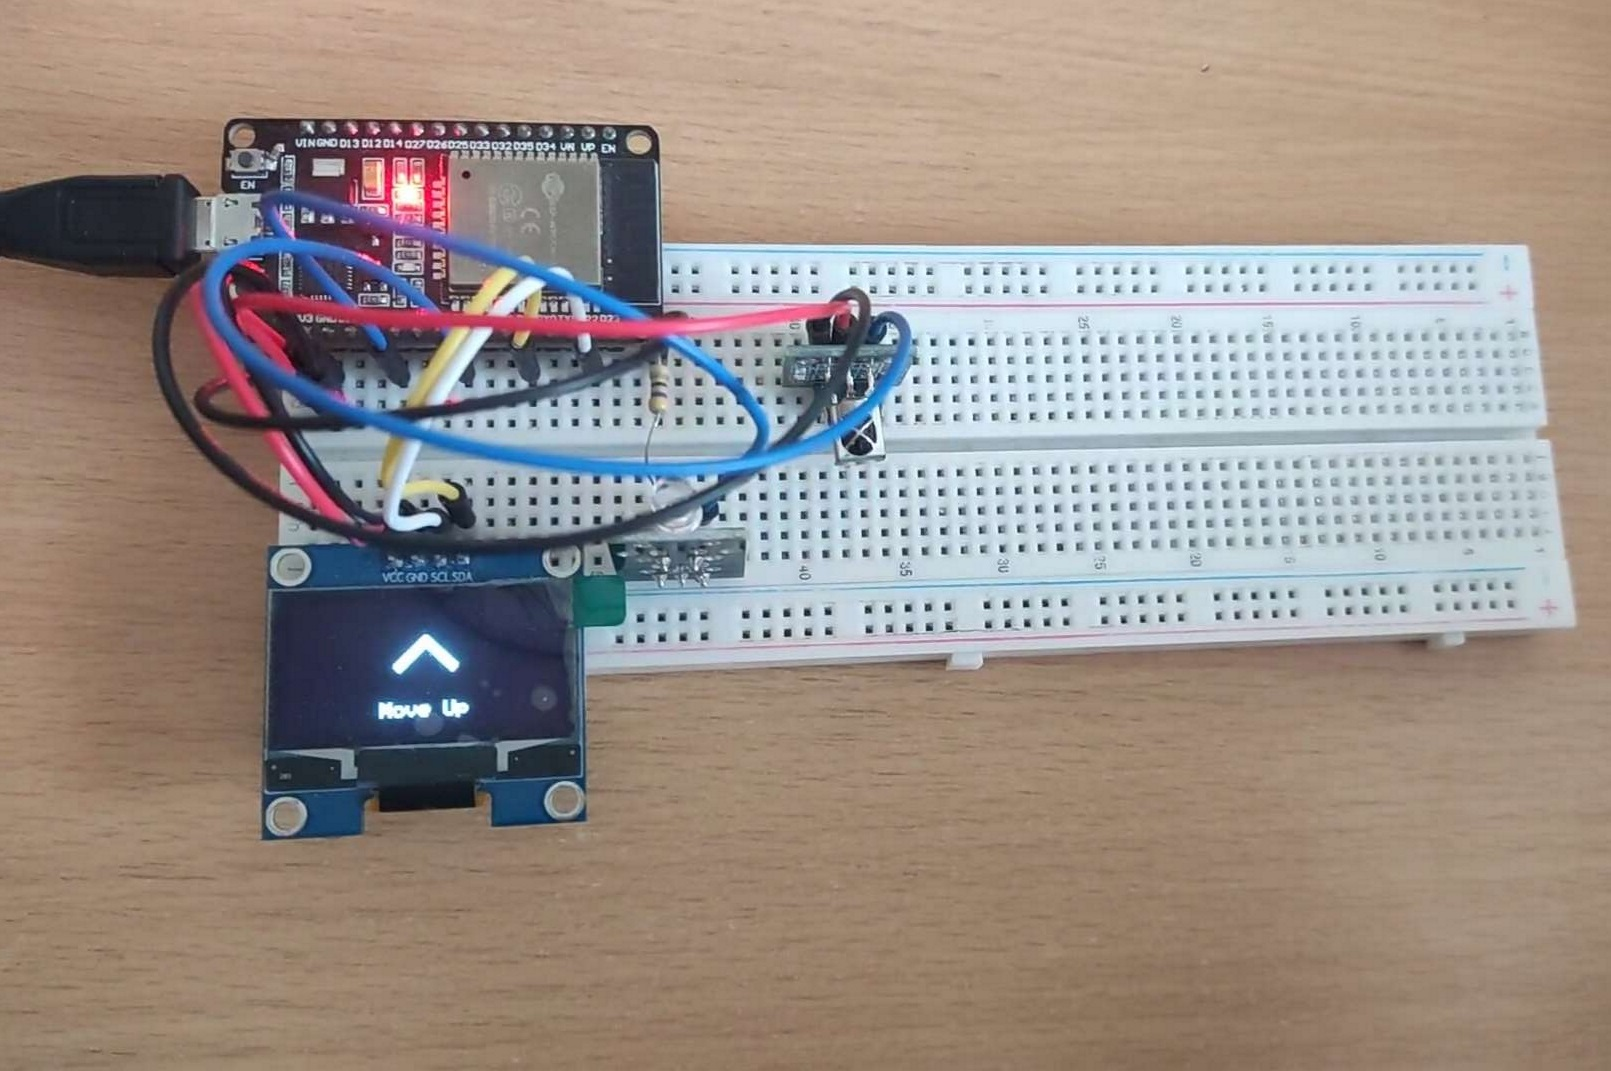
\includegraphics[width=14cm]{images/drawMoveUp.jpg}
   \caption{Wynik wywołania metody rysującej strzałkę w górę z opisem na wyświetlaczu}
   \label{Fig:drawMoveUp}
\end{figure}

\clearpage

\section{Aplikacja sterująca telewizorem}
\subsection{Struktura aplikacji}
Aplikacja mobilna została przygotowana przy pomocy frameworka Flutter i edytora kodu Visual Studio Code. Flutter jako narzędzie programistyczne udostępnia wygodny sposób dzielenia interfejsu użytkownika na ekrany i został on wykorzystany w aplikacji pilota. Wydzielono w projekcie główną stronę aplikacji odpowiedzialną za wyświetlanie jej nazwy, czyli ,,Bluetooth2IR'', oraz nawigowanie pomiędzy utworzonymi ekranami funkcjonalnymi. Elementy interfejsu zarządzane przez nią zostały wskazane na Rys. \ref*{Fig:mainPageElements} zawierającym okrojony zrzut ekranu z apliakjci mobilnej. Strona ta, zaimplementowana w pliku ,,homepage.dart'' jest głównym widgetem utworzonej aplikacji uruchamianej w ,,main.dart''. Plik wywołujący zbudowaną z widgetów aplikację oprócz samego jej uruchomienia definiuje także domyślne style czcionki, kolorów, przycisków i tła.
\begin{figure}[ht]
   \centering
   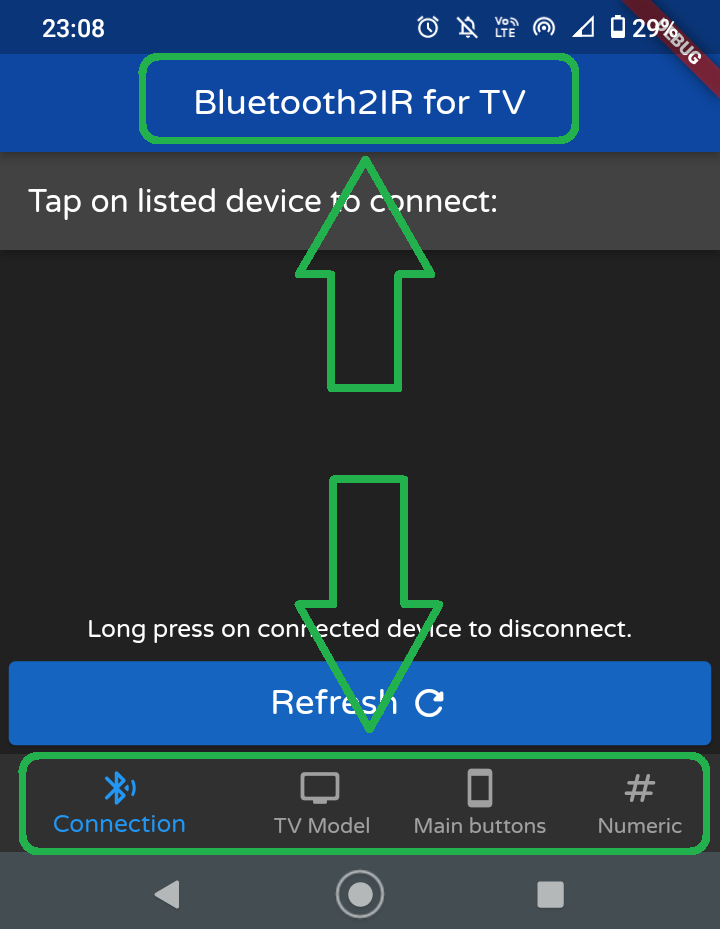
\includegraphics[width=8cm]{images/mainPageElements.png}
   \caption{Elementy interfejsu użytkownika zarządzane przez główną stronę aplikacji mobilnej pilota}
   \label{Fig:mainPageElements}
\end{figure}

Dolna część interfejsu użytkownika odpowiada za przemieszczanie się po ekranach aplikacji. Znaleźć tam można 4 elementy:
\begin{enumerate}[label=\alph*), leftmargin=1.25cm]
   \item Ekran ,,Connection'' - działający jako panel łączenia się aplikacji mobilnej pilota z urządzeniem pośredniczącym
   \item Ekran ,,TV Model'' - udostępniający wybór modelu telewizora, którym użytkownik chce sterować oraz możliwość modyfikacji i tworzenia własnych modeli
   \item Ekran ,,Main buttons'' - udostępniający różne najczęściej używane przyciski pilota
   \item Ekran ,,Numeric'' - udostępniający przyciski cyfr pilota
\end{enumerate}

\subsection{Moduł obsługujący BLE}
Aby skutecznie zarządzać połaczeniem BLE z urządzeniem pośredniczącym w zaprojektowanej aplikacji utworzono moduł o nazwie ,,BLEService'', w postaci klasy opartej o wzorzec Singleton, korzystający z biblioteki Flutter Blue Plus\cite{flutterBluePlus}. Utworzona klasa udostępnia szereg typowych metod dla zarządznia połączeniem.

Chcąc nawiązać połączenie z urządzeniem pośredniczącym, najpierw należy odnaleźć wszystkie dostępne urządzenia w okolicy. Przed tym, jednak jeszcze trzeba się upewnić, że smartfon posiada włączony adapter BLE. W projektowanej klasie służy do tego metoda ,,initCheckingBleAdapter()'' przedstawiona na List. \ref*{Lst:checkBLE}. Dodaje ona subskyrpcję do strumienia sprawdzającego włączenie adaptera BLE, która jeśli wykryje, że adapter jest wyłączony, pyta jednokrotnie użytkownika czy jednak nie chce go włączyć.

\lstinputlisting[inputencoding=utf8/cp1250, language={C++}, caption={\protect\input{captions/checkBLE.txt}\protect\relax}, label={Lst:checkBLE}]{codes/checkBLE.cpp}

Skanowanie urządzeń dostępnych w okolicy wymaga jeszcze włączonej lokalizacji. Sprawdzanie tego warunku realizowane jest za pomocą metody ,,checkLocationEnabled()'' ukazanej na List. \ref*{Lst:checkLocation}. Sprawdza ona czy użytkownik posiada włączoną lokalizację i jeśli nie, pyta go czy nie chciałby jej włączyć.

\lstinputlisting[inputencoding=utf8/cp1250, language={C++}, caption={\protect\input{captions/checkLocation.txt}\protect\relax}, label={Lst:checkLocation}]{codes/checkLocation.cpp}

Mając dostępny sposób na sprawdzenie działania lokalizacji i adaptera BLE, można przystąpić do skanowania dostępnych urządzeń bezprzewodowych. Zadanie to pełni metoda ,,scanBleDevices()'' przedstawiona na List. \ref*{Lst:scanBLE}. Sprawdza ona najpierw dostępność lokalizacji dzięki wcześniej opisanej metodzie ,,checkLocationEnabled()'', a następnie dodaje subskrypcję do strumienia odnajdywanych dostępnych urządzeń zawierających w nazwie ,,Bluetooth2IR for TV''. W ten sposób aplikacja będzie monitorować dostępne urządzenia i zapisywać je do strumienia jeśli nastąpi ich skanowanie. Następnie, zależnie od tego czy wszystkie wcześniej wymienione niezbędene zasoby są dostępne, następuje 3 sekundowe skanowanie dostępnych urządzeń lub jest ono pomijane.

\lstinputlisting[inputencoding=utf8/cp1250, language={C++}, caption={\protect\input{captions/scanBLE.txt}\protect\relax}, label={Lst:scanBLE}]{codes/scanBLE.cpp}

Zakładając, że odnaleziono przynajmniej 1 urządzenie pośredniczące, klasa udostępnia możliwość połączenia się z nim za pomocą metody ,,connectToBleDevice()'', która sprawdza czy urządzenie posiada odpowiednie charakterystyki odbioru informacji o wciśniętym przycisku na pilocie. Realizowane jest to za pomocą sprawdzania UUID serwisu i charakterystyk. Jeśli każdy z atrybutów urządzenia pośredniczącego zgadza się z wymaganiami projektowanego systemu, urządzenie pozostaje z nim połączone (już samo sprawdzanie atrybutów BLE wymaga chwilowego nawiązania połączenia z tym urządzeniem). Posiadając nawiązane połączenie moduł programowy jest gotowy do wysyłania informacji o wciśniętym przycisku. Za wysył danych do urządzenia pośredniczącego odpowiadają 2 metody, jedna z nich to ,,sendIrCodeToDevice()'' zaprezentowana na List. \ref*{Lst:sendingBLE}. Wysyła ona do charakterystyki kodu IR przycisku, dane w postaci listy 8 bajtowych liczb całkowitych bez znaku (po wcześniejszym przekonwertowaniu liczby całkowitej na tę listę), a następnie czeka na odpowiedź o powodzeniu lub niepowodzeniu transmisji. Tak zrealizowany wysył danych zpobiega nakładaniu się żądań zapisu do charakterystyk.

\lstinputlisting[inputencoding=utf8/cp1250, language={C++}, caption={\protect\input{captions/sendingBLE.txt}\protect\relax}, label={Lst:sendingBLE}]{codes/sendingBLE.cpp}


\subsection{Ekran łączenia się z urządzeniem pośredniczącym poprzez BLE}
Ekran nawiązywania połączenia z urządzeniem pośredniczącym został oparty o moduł ,,BLEService'' opisany w poprzednim podpunkcie. Zawiera on właściwie jedynie przycisk odświeżania dostępnych urządzeń w pobliżu oraz interaktywną listę wyświetlającą te urządzenia.
Przełączając się na ten ekran lub włączając aplikację, gdyż jest on domyślnym pod-ekranem startowym, użytkownik uruchomi sprawdzanie włączenia adaptera BLE oraz lokalizacji. Stanie się tak, ponieważ zaimplementowane zostało automatyczne uruchamianie skanowania, które wymaga wymienionych zasobów do poprawnego działania, a metoda inicjalizacji tego obiektu zajmuje się sprawdzeniem ich dostępności. Ekrany aplikacji przedstawiające zapytania o włączenie lokalizacji oraz modułu Bluetooth, a także ekran podczas wyszukiwania dostępnych urządzeń zostały przedstawione na Rys. \ref*{Fig:initBLE}.
\begin{figure}[ht]
   \centering
   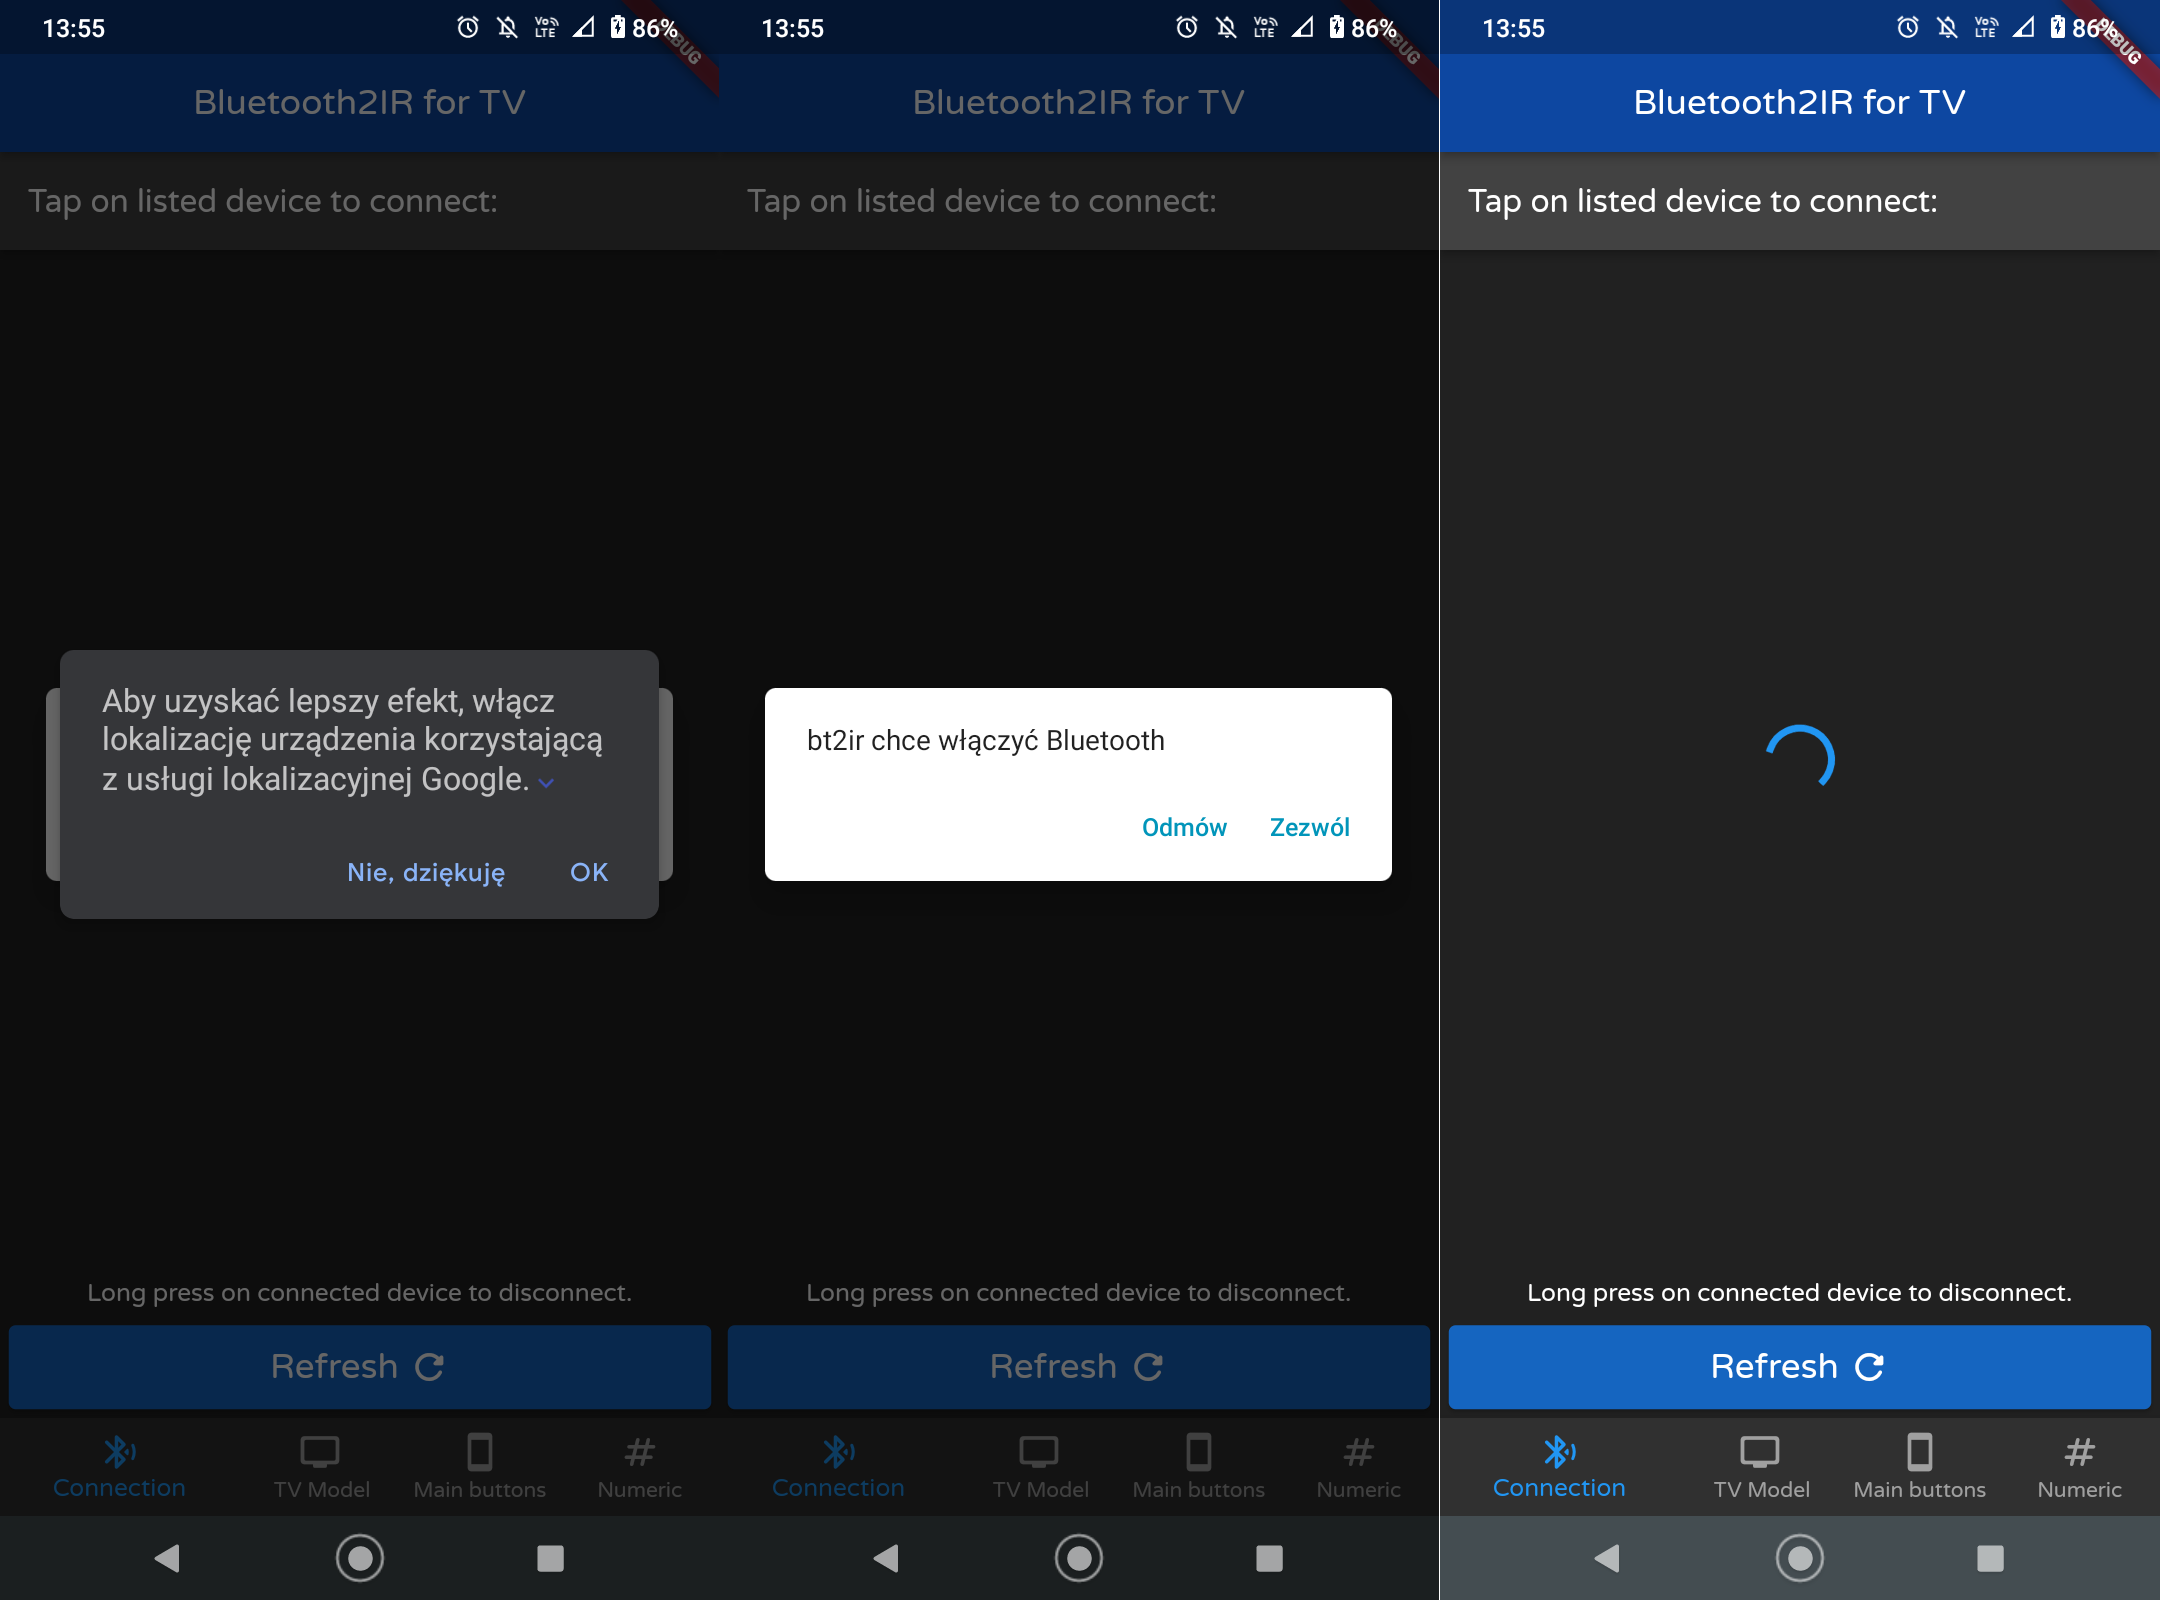
\includegraphics[width=14cm]{images/initBLE.png}
   \caption{Ekrany kolejno zapytania o włączenie lokalizacji, adaptera Bluetooth oraz ekranu podczas skanowania dostępnych urządzeń BLE}
   \label{Fig:initBLE}
\end{figure}

Jeśli użytkownik włączył swoje urządzenie pośredniczące i jest ono w pobliżu, a także w aplikacji nastąpiło poprawne skanowanie, zobaczy on swoje urządzenie na liście dostępnych urzadzeń pod nazwą ,,Bluetooth2IR for TV''. Element listy zawiera nazwę urządenia pośredniczącego, jego adres w postaci liczby szesnastkowej oraz ikonę ułatwiającą zroumienie co znajduje się w tym elemencie. Użytkownik może się połączyć z  tak odnalezionym urządzeniem za pomocą kliknięcia na nie na liście. Podczas nawiązywania połączenia element zyska niebieskie podświetlenie i znacznik ładowania, a po połączeniu podświetlenie stanie się zielone i pojawi się na tym elemenecie ikona Bluetooth. Kiedy użytkownik już zakończy pracę z pilotem lub będzie chciał się przełączyć na inne urządzenie, może rozłączyć się z aktualnie połączonym urządzeniem za pomocą przytrzymania elementu, który go dotyczy. Ekran przedstawiający odnalezione urządzenie znajdujące się na liście dostępnych oraz jego stan po rozpoczęciu nawiązywania połączenia, a także po poprawnym  połączeniu się z tym urządzeniem znajdują się na Rys. \ref*{Fig:connectBLE}.

\begin{figure}[ht]
   \centering
   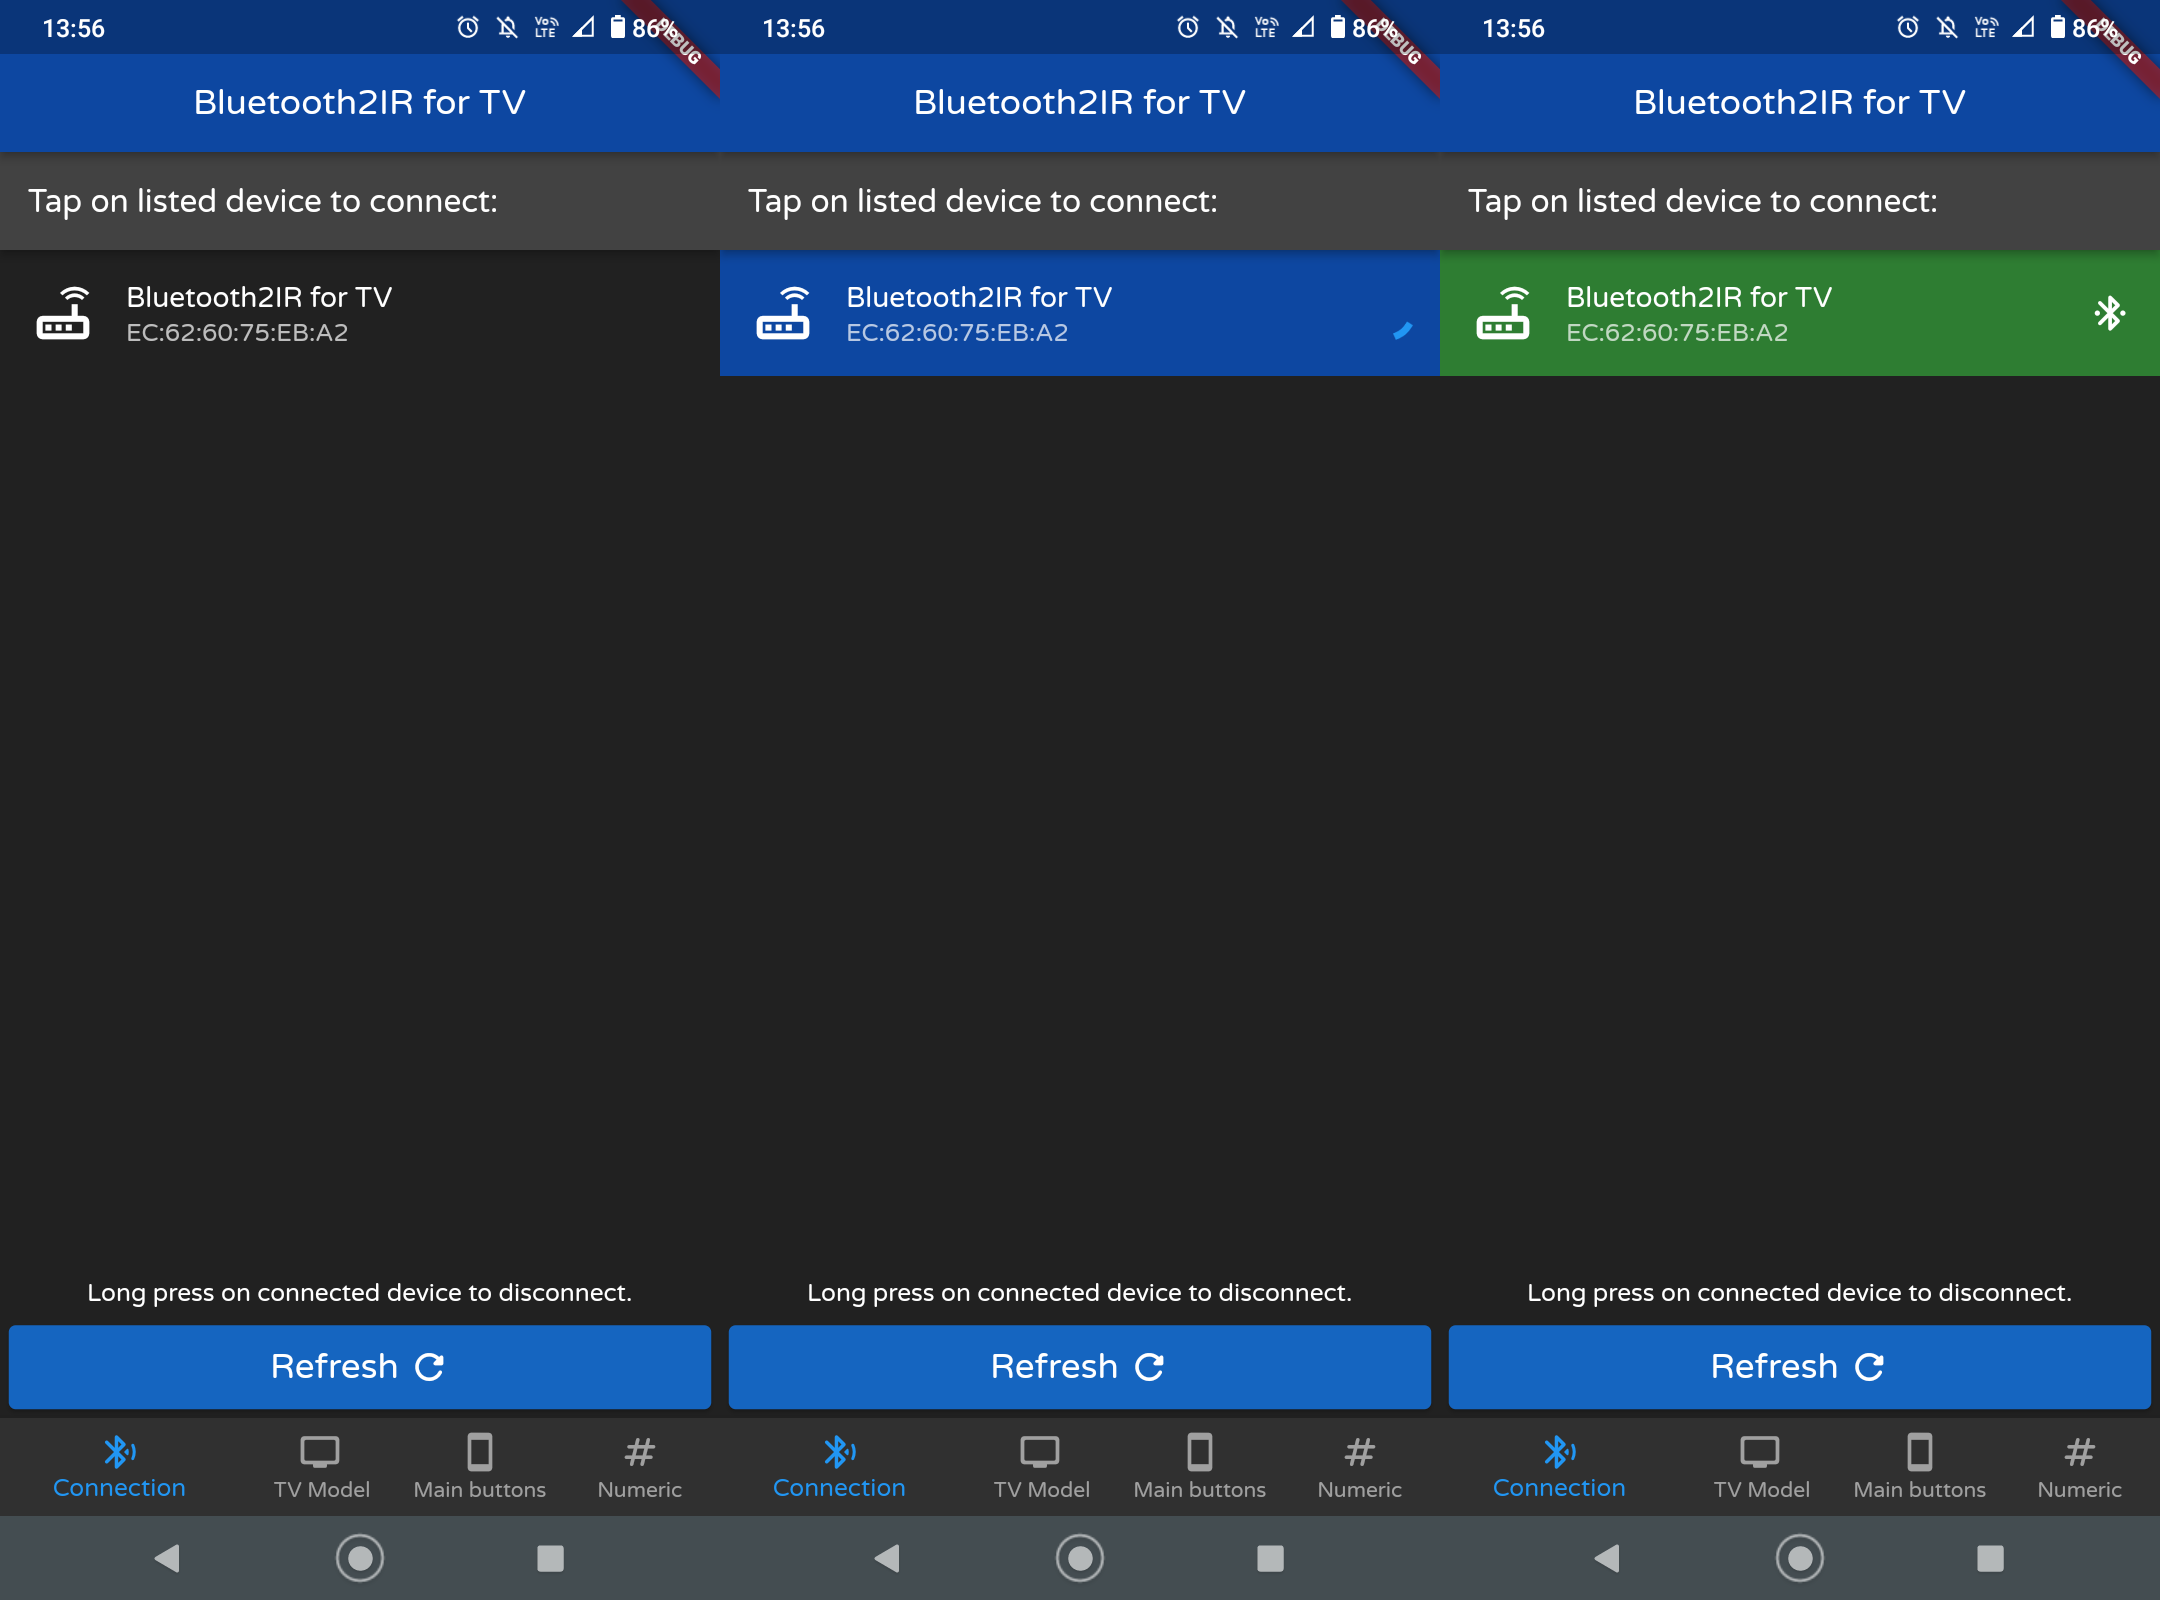
\includegraphics[width=14cm]{images/connectBLE.png}
   \caption{Ekrany kolejno po odnalezieniu urządzenia pośredniczącego, po rozpoczęciu łączenia z nim oraz po połaczeniu za pomocą BLE}
   \label{Fig:connectBLE}
\end{figure}

\subsection{Moduł obsługi przechowywania zestawów przycisków}
W aplikacji mobilnej pilota uniwersalnego użtykownik ma możliwość wyboru modelu telewizora, którym chce sterować. Aby reprezentować programowo zbiór zdefiniowanych modeli telewizorów i przypisanych do nich parametrów przycsików  oraz zrealizować zapamiętywanie tych zestawów pomiędzy uruchomieniem aplikacji utworzono moduł ,,tv\_model.dart''. Odpowiedzalny jest on za zdefiniowanie klasy danych opisujących pojedynczy przycisk pilota, oraz składającej się z zbioru pól o typie takich przycisków, klasy pełnego zestawu przycisków pilota służącego do sterowania danym modelem telewizora. 

Klasa ,,Button'' odpowiadająca za reprezentację  pojedynczego przycisku zawiera informacje w postaci pól prywatnych o typie przycisku i opdowiadającemu mu kodzie IR. Udostępnia także 2 metody: ,,fromJson()'' i ,,toJson()''. Pozwalają one na zapis i odczyt danych tekstowych w fromacie JSON, reprezentujących obiekty wspomnianej klasy. Dzięki tym metodom, typy danych używające tej abstrackcji przycisku mogą nie martwić się o jej konwerjsę do tego fromatu i swobodnie przeprowadzać zapis do plików tekstowych struktur, złożonych z obiektów klasy ,,Button''. Iplementacja tych metod znajduje się na List. \ref*{Lst:buttonJson}.
\lstinputlisting[inputencoding=utf8/cp1250, language={C++}, caption={\protect\input{captions/buttonJson.txt}\protect\relax}, label={Lst:buttonJson}]{codes/buttonJson.cpp}

Z kolei klasa TVModel składa się z wielu obiektów klasy Button z odpowiednio zdefniowanymi typami przycisku w postaci numerycznej. Posiada też pole nazwy modelu telewizora, którym definiowane przyciski na pilocie mają sterować. Dla tej klasy przeładowano także operator porównania który uwzględnia jedynie nazwę modelu telewizora co było wymagane dla używania tego typu danych w zbiorze niepowtarzających się danych ,,Set''. Posiada ona także metody toJson() oraz fromJson(), które dla pojedynczego obiektu zestawu przycisków są ciągami wywołań tego rodzaju metod z klasy Button i zapisu nazwy modelu sterowanego telewizora. 

Chcąc teraz przechowywać dane pomiędzy uruchomieniami aplikacji można skorzystać z nieulotnej pamięci aplikacji, do której można uzyskać dostęp za pomocą klasy SharedPreferences[] udostępnianego przez framework Flutter. Sama klasa z frameworka daje bezpośredni dostęp do pamięci aplikacji Androida w postaci klasy języka Dart. Dla wygody i zkonsolidowania operacji wykonywanych na tym obiekcie utoworzono klasę SharedPrefs służącą jako interfejs dostępu do danych zapisanych w pamięci oraz udostępniający łatwe w użyciu metody operujące właśnie na zestawach przycisków dla modeli telewizorów. Klasa ta przechowuje instancję obiektu SharedPreferences, która jest inicjowana za pomocą metody ,,initialize()'', oraz udostępnia statyczne metody pozwalające zapisywać i odczytywać nawet całe listy zestawów przycisków. Część definicji tej klasy zawierającą pole przechowujące instancę obiektu SharedPreferences, metodę inicjalizującą ten obiekt oraz metody zapisujące i odczytujące listy zestawów przycisków zawarto na List. \ref*{Lst:sharedPrefs}

\lstinputlisting[inputencoding=utf8/cp1250, language={C++}, caption={\protect\input{captions/sharedPrefs.txt}\protect\relax}, label={Lst:sharedPrefs}]{codes/sharedPrefs.cpp}

Statyczna metoda do zapisu danych w nieulotnej pamięci aplikacji ,,saveTVModels()'' przyjmuje w argumencie listę zestawów przycisków. Oczekuje najpierw na otrzymanie instancji obiektu klasy SharedPreferences. Kolejno dalej przy pomocy odpowiednich metod tworzy łańcuch tekstowy  reprezentujący wszystkie dane zawarte w podanej do funkcji liście przy pomocy formatu JSON. Tak utworzony łańcuch jest zapisywany do szufladki zawierającej tekst w pamięci o nadanej jej nazwie ,,tvModels''.

Odczyt danych z nieulotnej pamięci aplikacji odbywa się za pomocą metody ,,getTVModels()''. Jak metoda zapisująca dane, najpierw upewnia się ona, że dostępna jest instancja klasy SharedPreferences. Następnie pobierany jest z pamięci łańcuch znakowy zawarty w szufladce o nazwie ,,tvModels'', przechowjący dane listy zestawów przycisków w formacie JSON.
Kolejno dalej dekodowany jest ten łańcuch do listy obiektów JSON, by końcowo przekonwertować te dane do obiektów klasy ,,TVModel'' przy pomocy mapowania właśnie na ten typ danych.

\subsection{Ekran wyboru i edycji zestawu przycisków dla konkretnego modelu telewizora}
Drugi ekran o nazwie ,,TV Model'' daje użytkownikowi możliwość wyboru zestawu  predefiniowanych przcisków dla danego modelu telewizora lub utworzenia czy edytowania własnego zestawu. W pierwszej chwili po przejściu na ten ekran ładowane są zapamiętane zestawy przycisków z nieulotnej pamięci apliakacji. Tak załadowane zestawy przycisków stają się pozycjami pola wyboru modelu telewizora, którym użytkownik chce sterować. 

Jeśli to pierwsze uruchomienie tego ekranu korzystający z aplikacji ujrzy na liście wybrany pusty zestaw przycików przyjazny do tworzenia własnego zestawu. Może on wtedy wybrać predefiniowany zestaw ,,Manta'' i przejść do korzystania z przycisków pilota w kolejnych ekranach. Stan aplikacji po pierwszym przejściu do tego ekranu i po wybraniu predefiniowanego modelu Manta został przedstawiony na Rys.\ref*{Fig:choosingManta}.
\begin{figure}[ht]
   \centering
   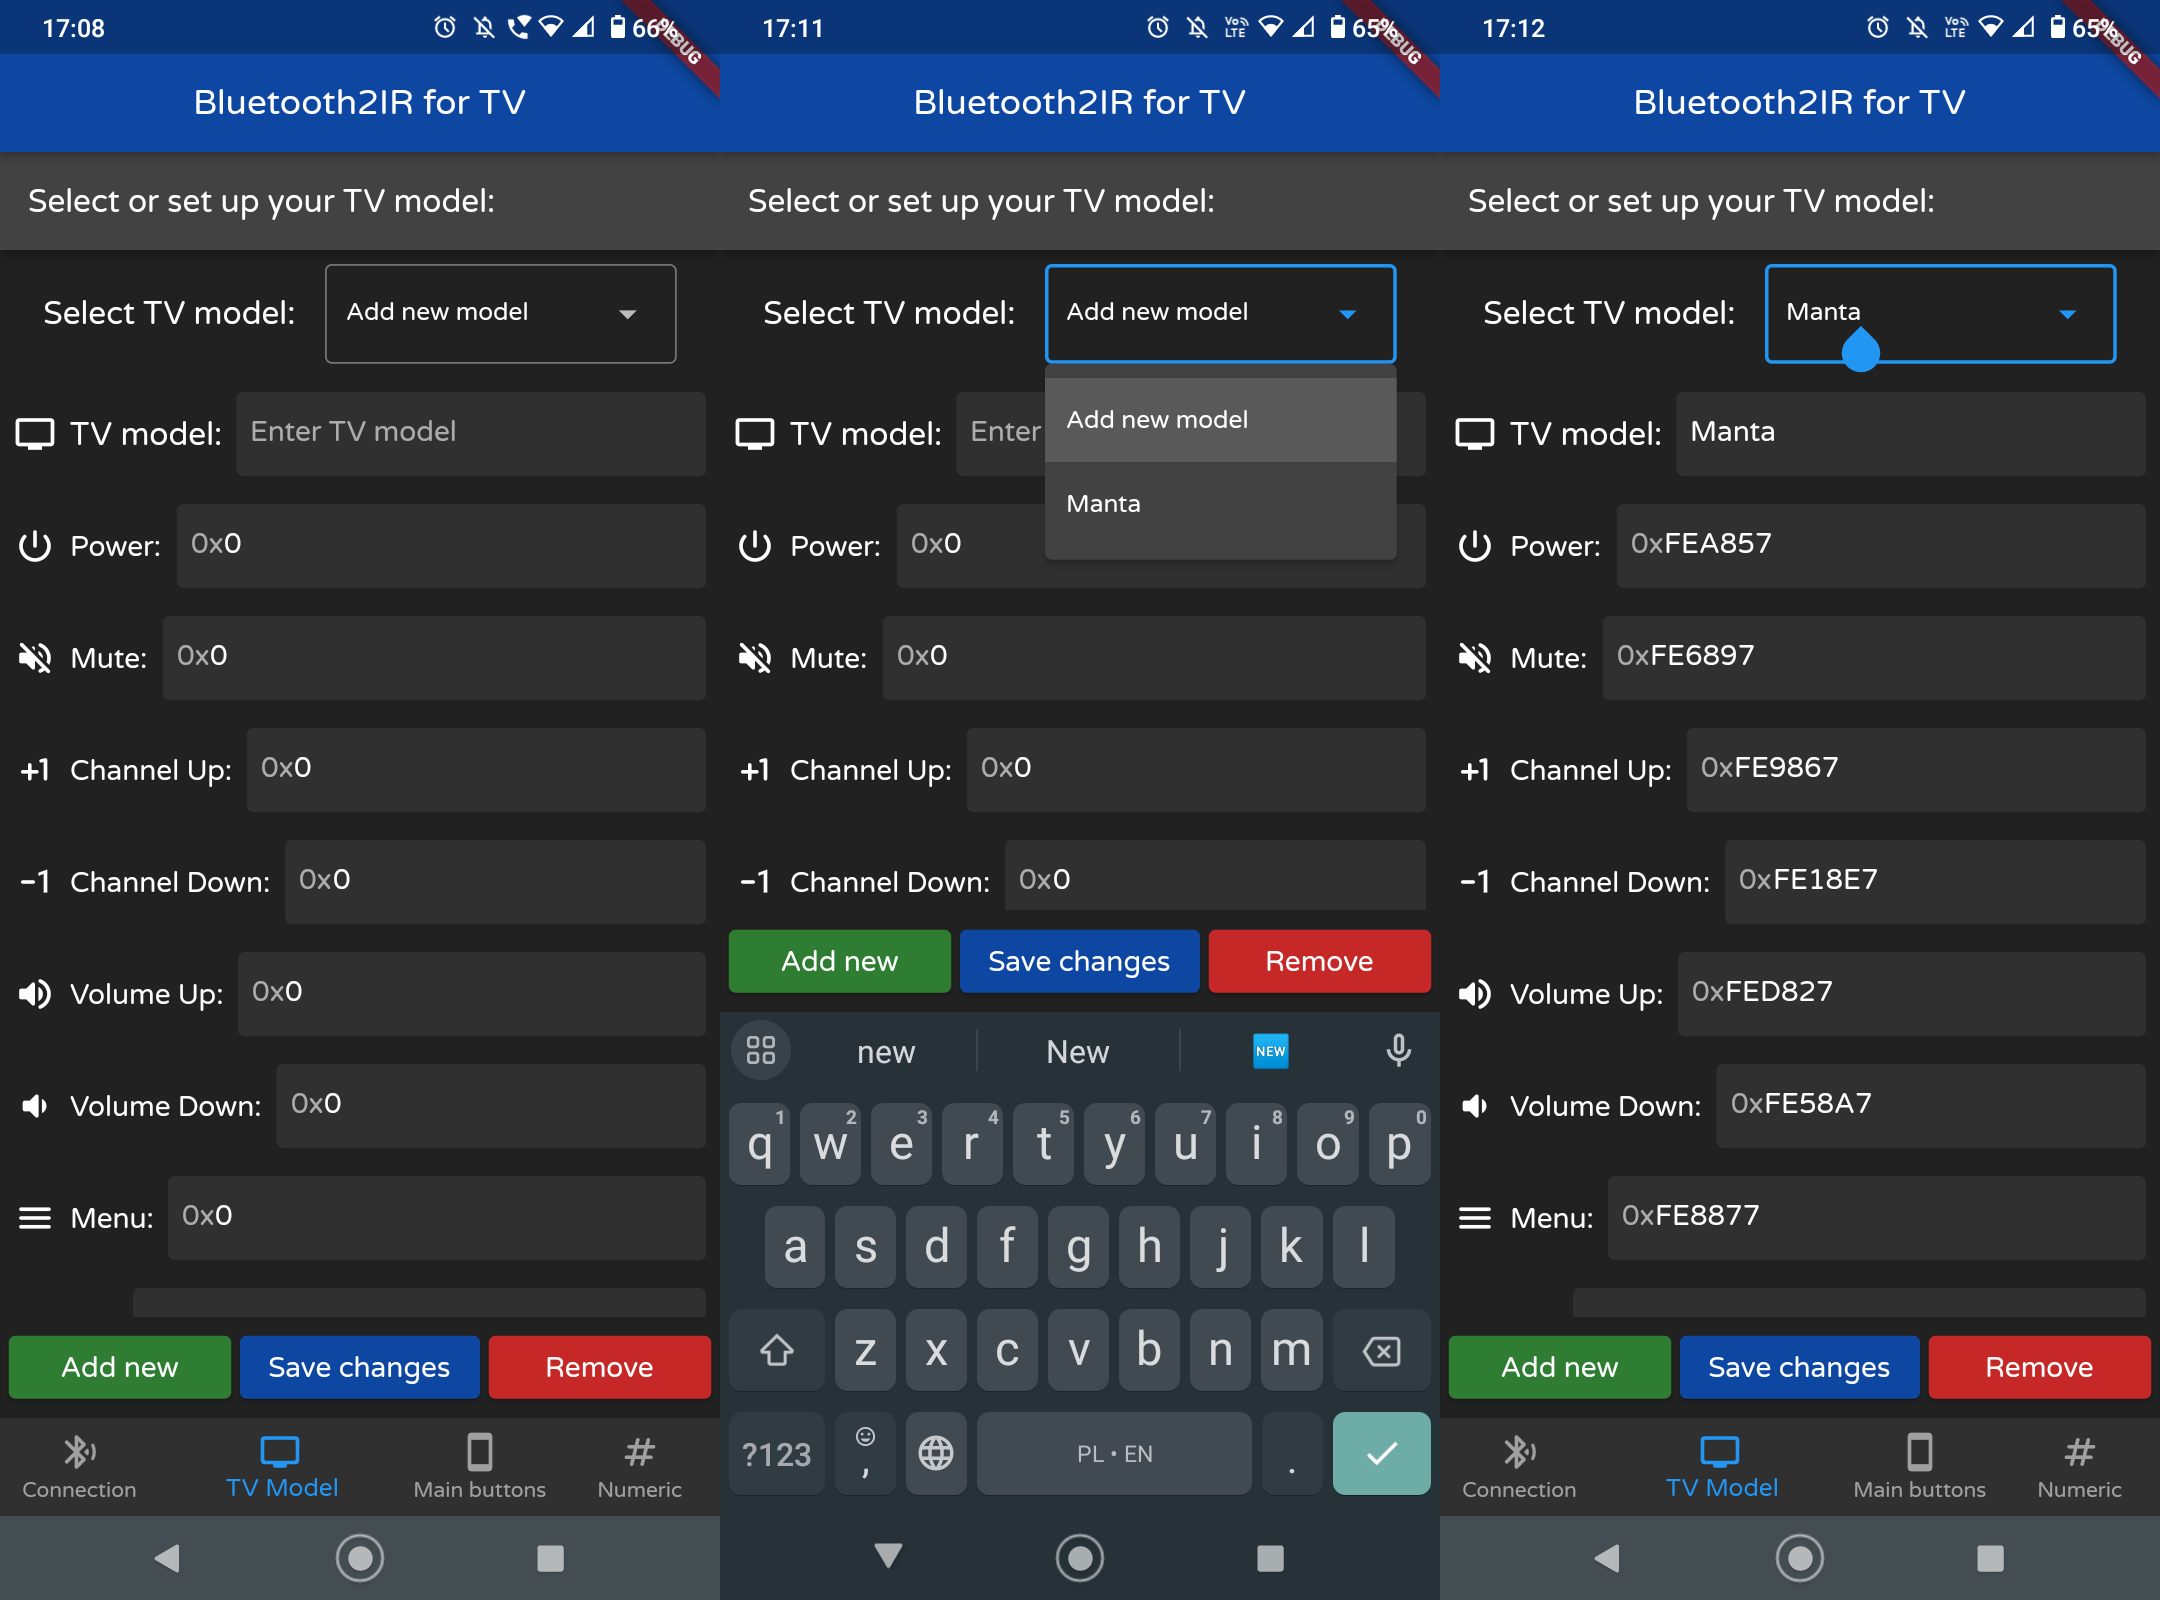
\includegraphics[width=14cm]{images/choosingManta.png}
   \caption{Ekrany aplikacji kolejno po przełączeniu na ekran ,,TV Models'', po rozwinięciu listy, oraz po wybraniu modelu ,,Manta''}
   \label{Fig:choosingManta}
\end{figure}

Ważnym elementem tego ekranu jest także możliwość dodania nowego zestawu przycisków sterujących telewizorem. Można tego dokonać najlepiej za pomocą wybrania pozycji ,,Add new Model'', ale nie jest to wymóg. Wystarczy, że nowa wprowadzona podczas edycji nazwa modelu nie będzie się jeszcze znajdować na liście dostępnych modeli. Wybierając więc jakąś pozycję i edytując jej pola według uznania, koniecznie zmieniając nazwę modelu, możemy utworzyć nowy zestaw. Należy pamiętać jednak aby wpisać poprawną liczbę w fromacie heksadecymalnym bo w przeciwnym wypadku fromularz zwróci błąd i nie uda się dodać tak skonfigurowanego zestawu. Przykład takiego procesu dla nowego modelu on nazwie ,,Samsung'' został przedstawiony na Rys. \ref*{Fig:addingSamsung}.

\begin{figure}[ht]
   \centering
   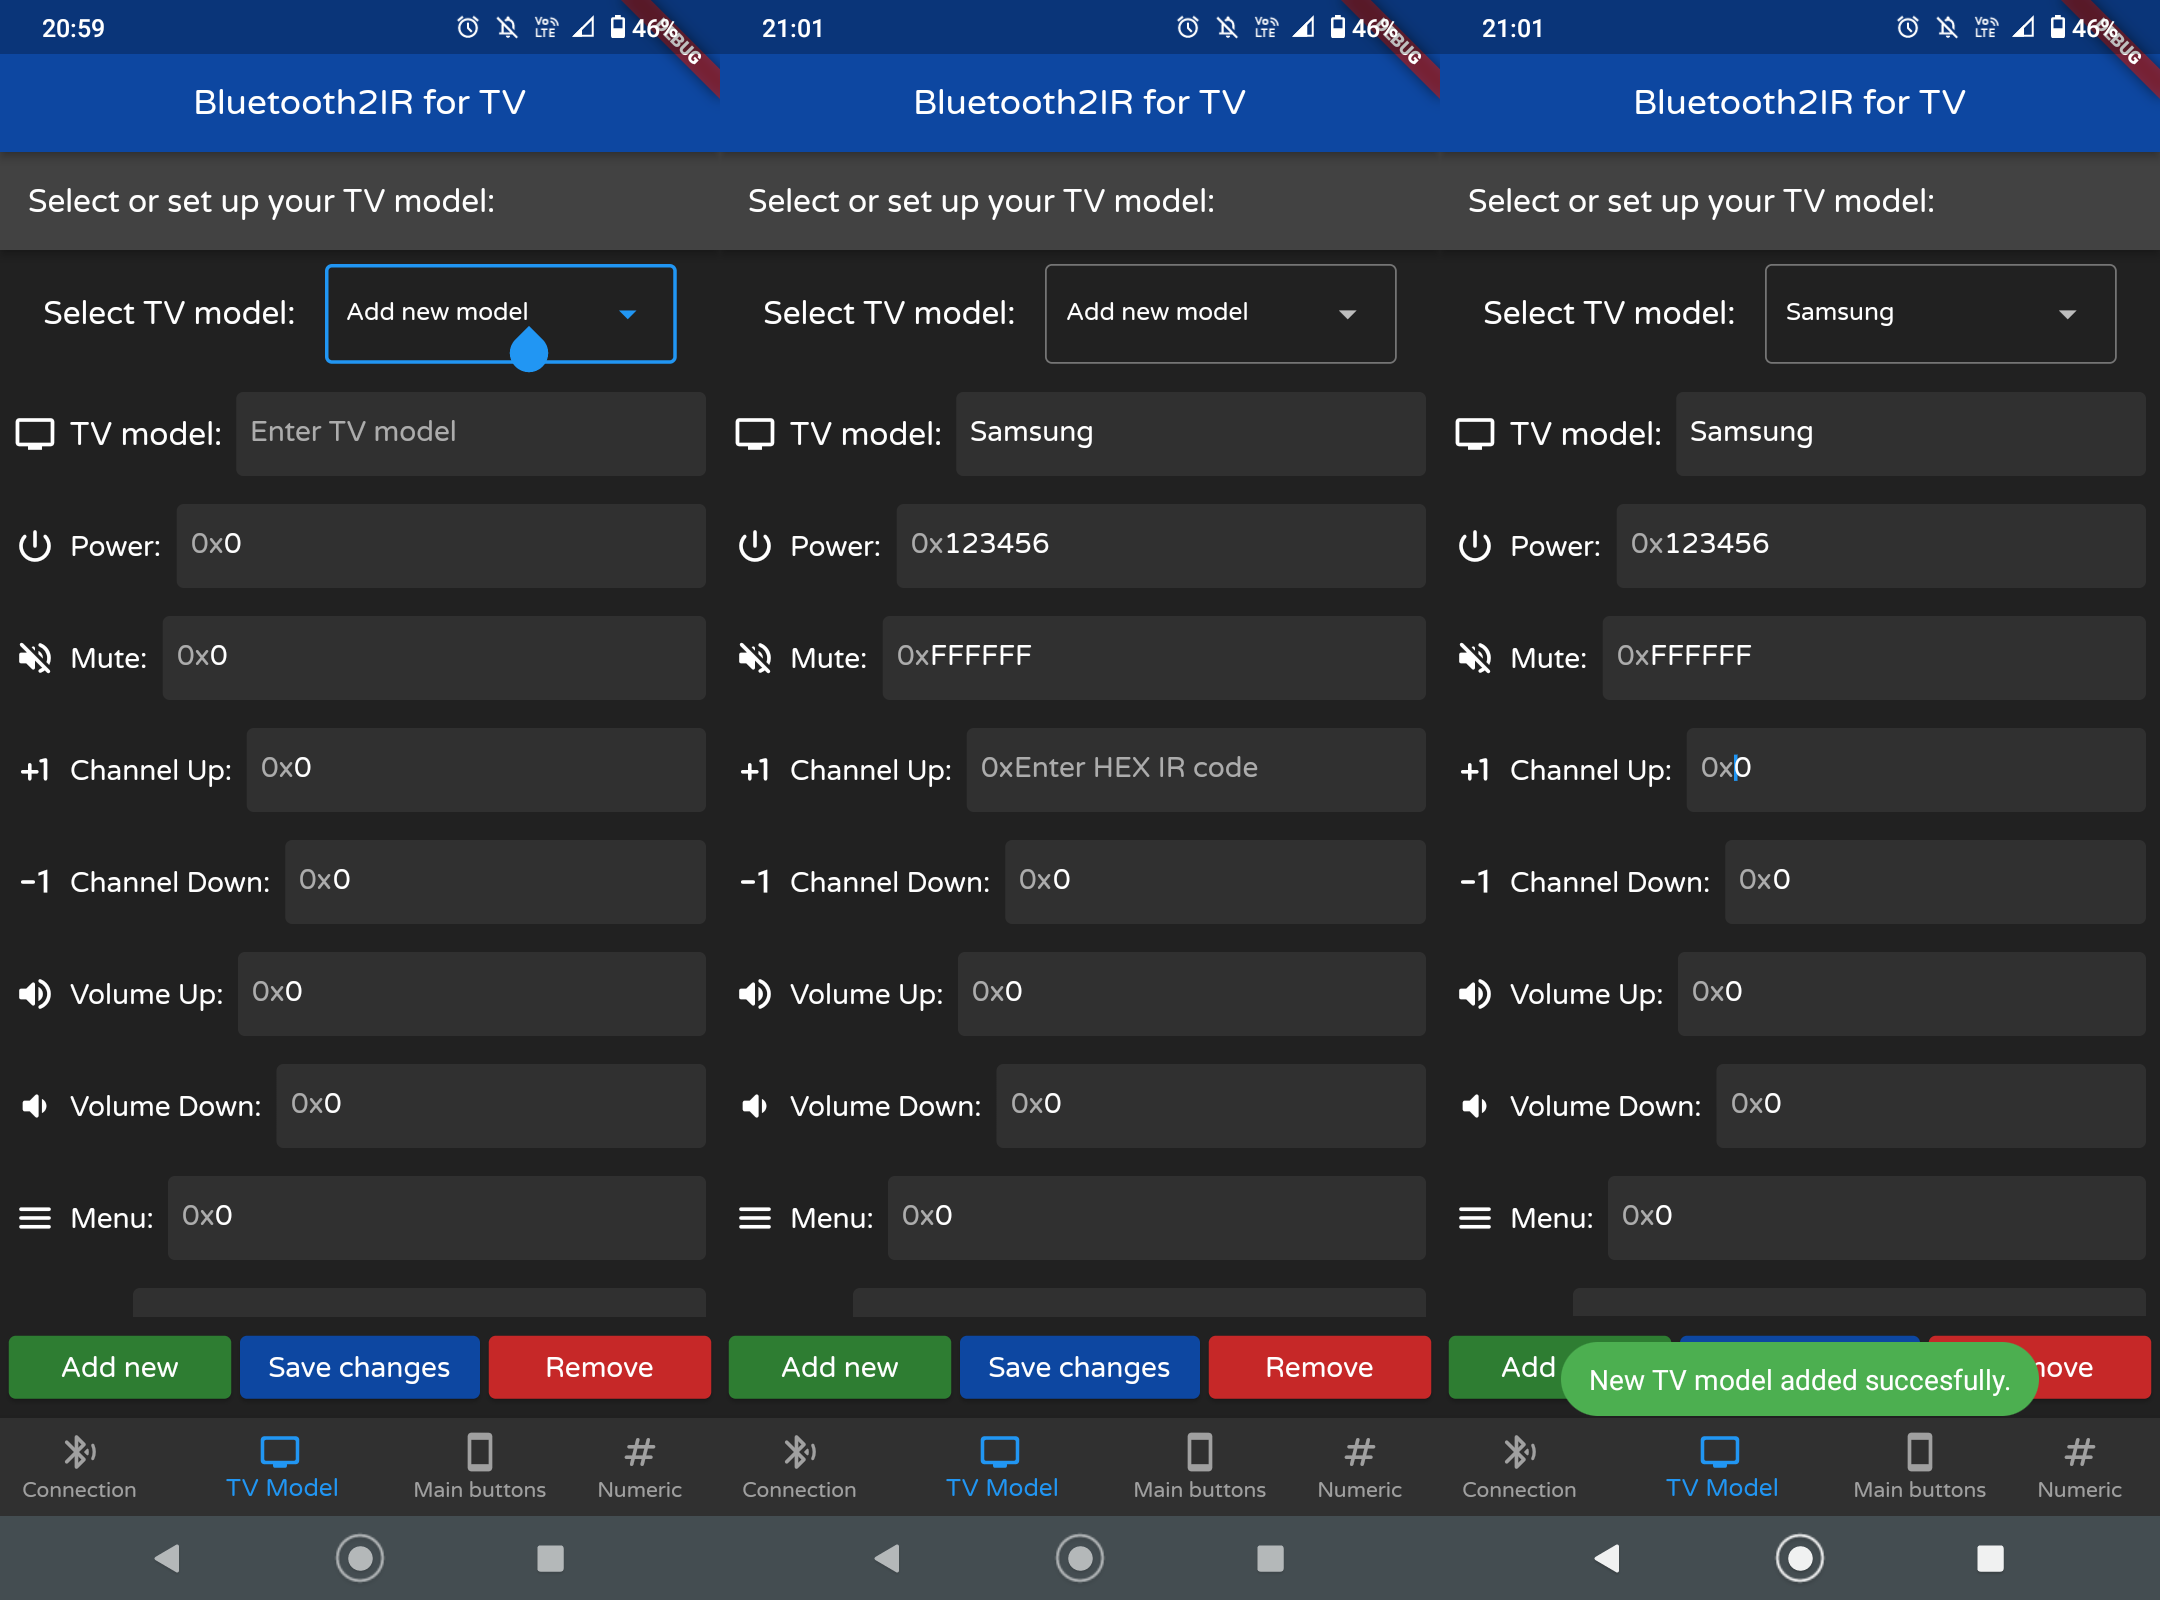
\includegraphics[width=14cm]{images/addingSamsung.png}
   \caption{Ekrany aplikacji kolejno po przełączeniu na ekran ,,TV Models'', po zmianie nazwy modelu oraz wybranych kodów przycisków, oraz dodaniu nowego modelu ,,Samsung''}
   \label{Fig:addingSamsung}
\end{figure}

Edycja utworzonego przez użytkownika zestawu przycisków jest równie prosta. Wybiera on najpierw element, który chce edytować, zmienia w nim dane według uznania zachowując jednak ich poprawność formatu. Korzystający nie może jedank zmienić nazwy takiego modelu, a jeśli to zrobi informowany jest o niepowodzeniu i proponowane jest mu skorzystanie z opcji ,,Add new''. Edycję modelu ,,Samsung'', jej zakończenie oraz  próbę zmiany nazwy tego modelu przedstawiono na Rys.\ref*{Fig:changingSamsung}.

\begin{figure}[ht]
   \centering
   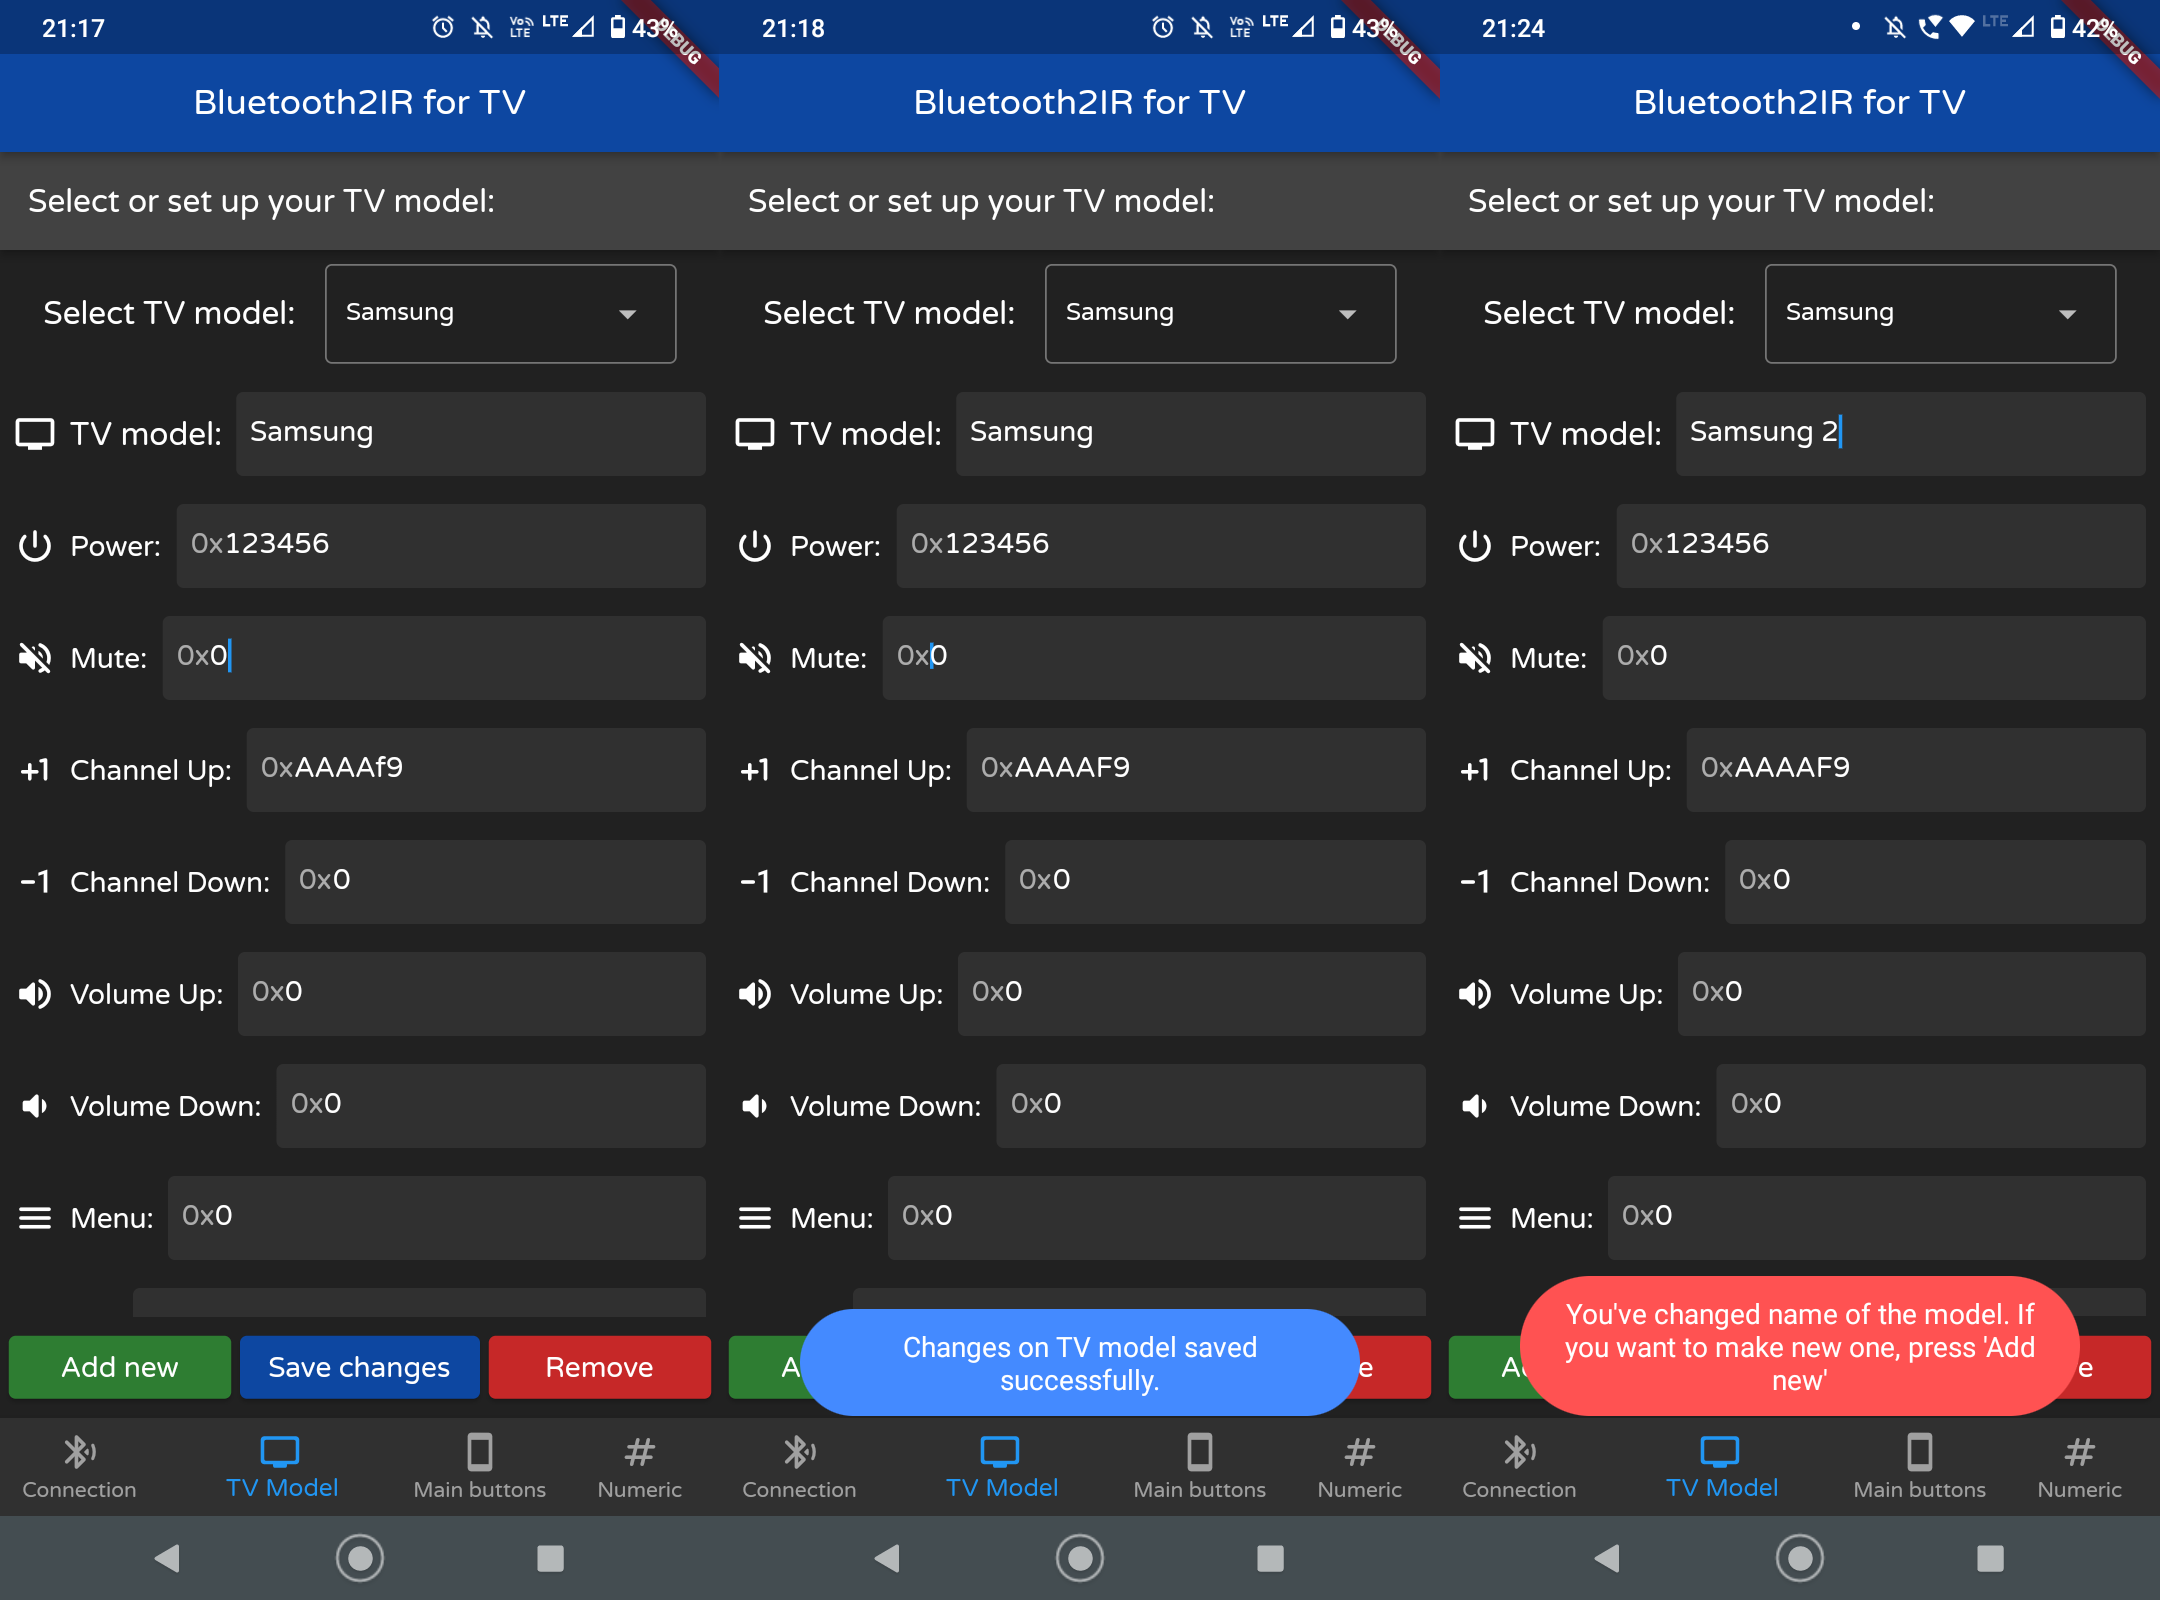
\includegraphics[width=14cm]{images/changingSamsung.png}
   \caption{Ekrany aplikacji kolejno po edycji modelu ''Samsung'', zatwierdzeniu tych zmian oraz próbie zmiany jego nazwy zakończonej niepowodzeniem}
   \label{Fig:changingSamsung}
\end{figure}

Usunięcie zestawu przycisku jest być może nawet zbyt proste. Wystarczy wybrać interesujący nas element z listy i kliknąć ,,Remove''. Jeżeli użtykownik spróbuje usunąć 2 podstawowe modele czyli pusty model oraz ,,Mantę'' zakończy się to niepowodzeniem. Sytuację poprawnego usunięcia zestawu dla modelu ,,Samsung'', oraz próby usunięcia zestawu ''Manta'' zakończonej niepowodzeniem przedstawiono na Rys. \ref*{Fig:removingSamsung}.

\begin{figure}[ht]
   \centering
   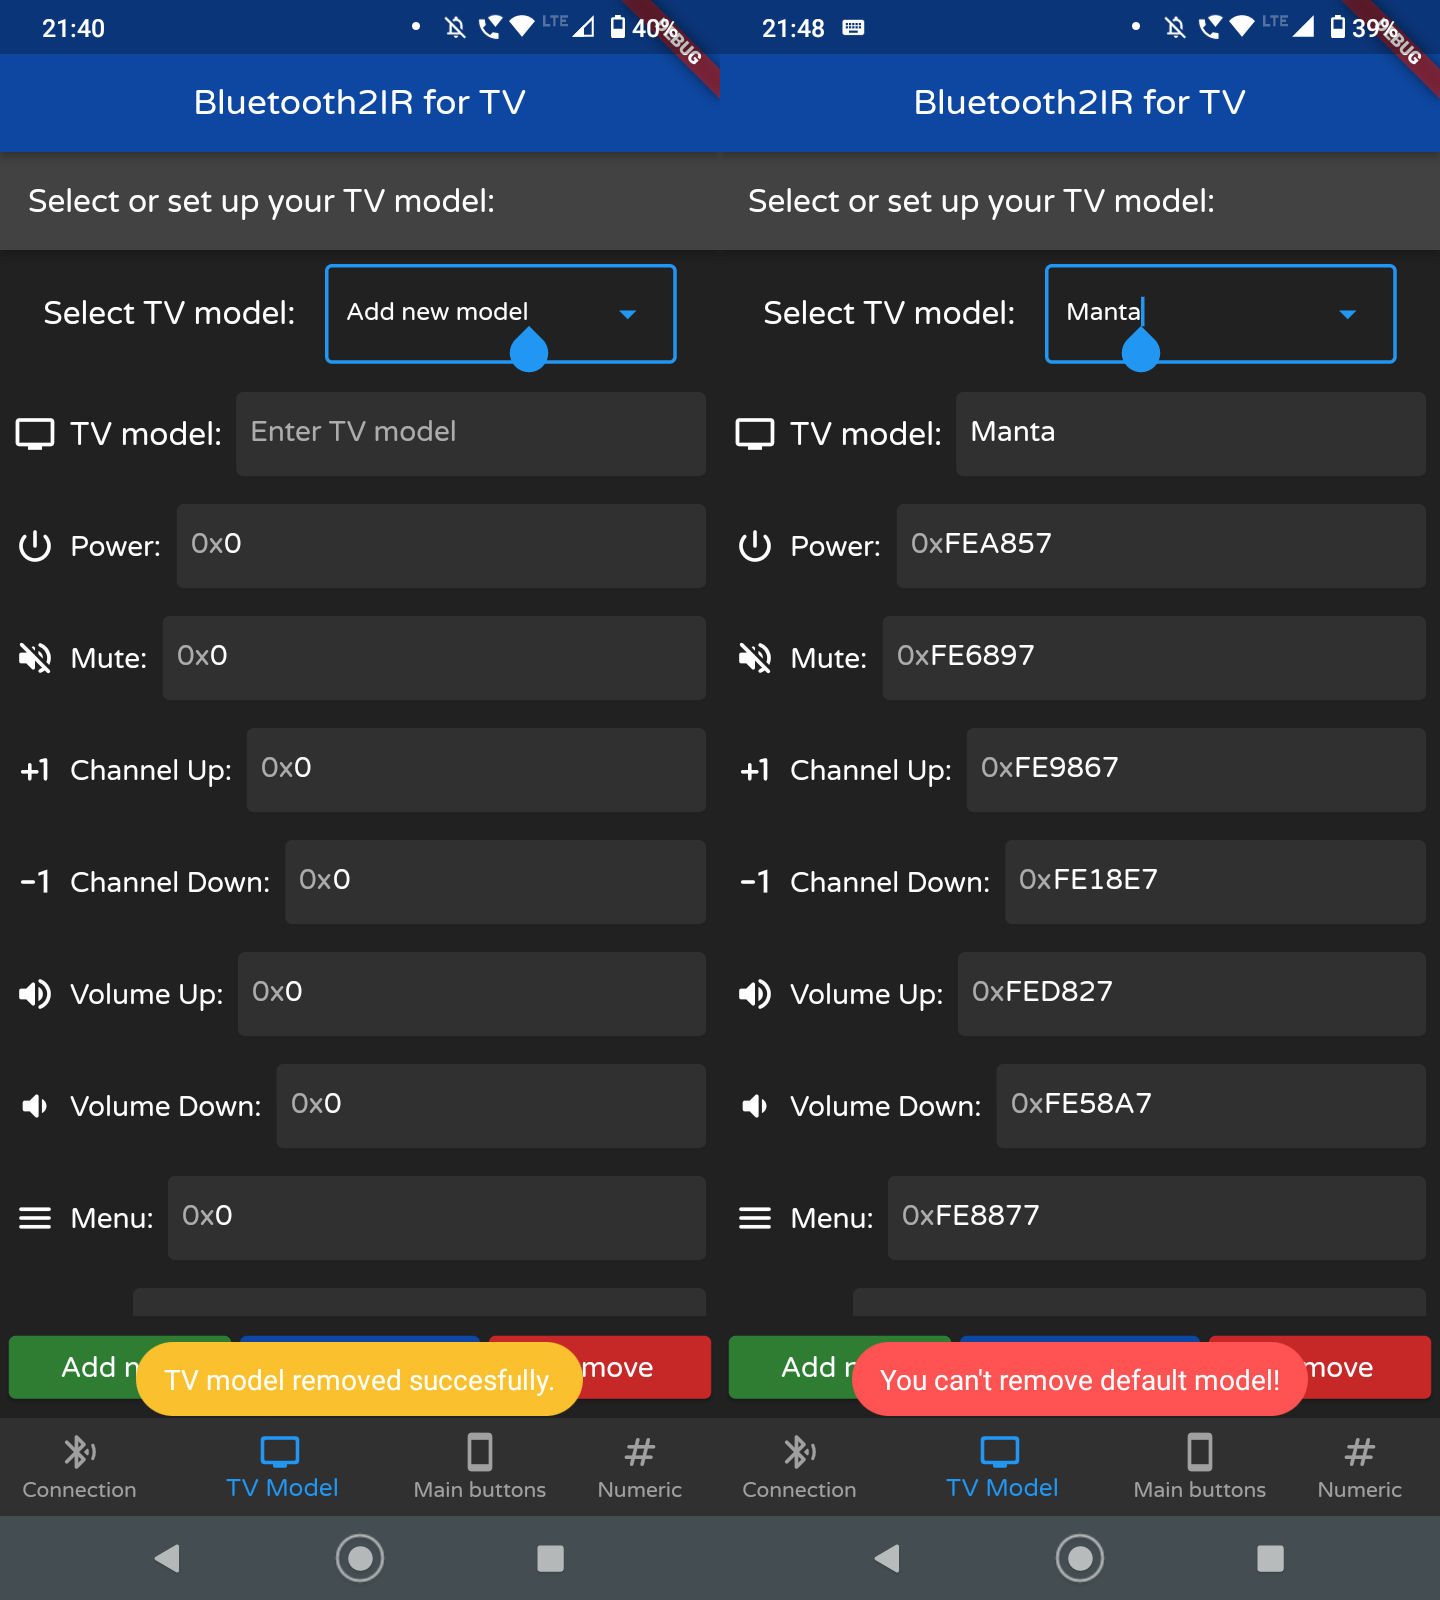
\includegraphics[width=10cm]{images/removingSamsung.png}
   \caption{Ekrany aplikacji kolejno usunięciu zestawu ''Samsung'' oraz próbie usunięcia zestawu ,,Manta'' zakończonej niepowodzeniem}
   \label{Fig:removingSamsung}
\end{figure}

Każda z przedstawionych funkcjonalności odczytywania i zapisywania danych jest zaimplementowana przy pomocy wcześniej omówionej klasy SharedPrefs i wykorzystaniu klas z pliku ,,tv\_model.dart''. Elementy edycyjne ekranu zostały zespolone za pomocą logiki formularza. Każde pole edycji posiada własny walidator danych. Pole nazwy wymaga jedynie nie pustego łańcucha tekstowego, a pola kodów IR, liczb w postaci szesnastkowej(poprawne są małe i wielkie litery). Podczas każdego wyboru innego zestawu przycisków, usunięciu jakiegoś czy dodaniu nowego zostaje aktualizowany globalny uchwyt do zestawu przycisków, dzięki któremu kolejne ekrany mogą korzystać z zdefiniowanych parametrów przycisków aktualnie wybranego zestawu.


\subsection{Ekrany przycisków pilota}
Aby użytkownik mógł finalnie skorzystać ze sterowania telewizorem, udostępnione zostały 2 ekrany. Pierwszy z nich o nazwie ,,Main Buttons'' zawiera najczęściej spotykane typy przycisków jak włączający telewizor, zmieniajacy głośność, kanał i im podobne. Przyciski na tym ekranie zostały rozmiesczone tak aby jak najbardziej imitować ich rozmieszczenie na zwykłym pilocie. 
Utworzony został również ekran pozwalający na wprowadzanie cyfr o nazwie ,,Numeric''. Zbudowany został tak, aby cyfry były jak największe na ekranie, a zarazem przyciski pozostały wygodne w użyciu. Wygląd obu ekranów w aplikacji przedstawiony został na Rys. \ref*{Fig:buttonScreens}.

\begin{figure}[ht]
   \centering
   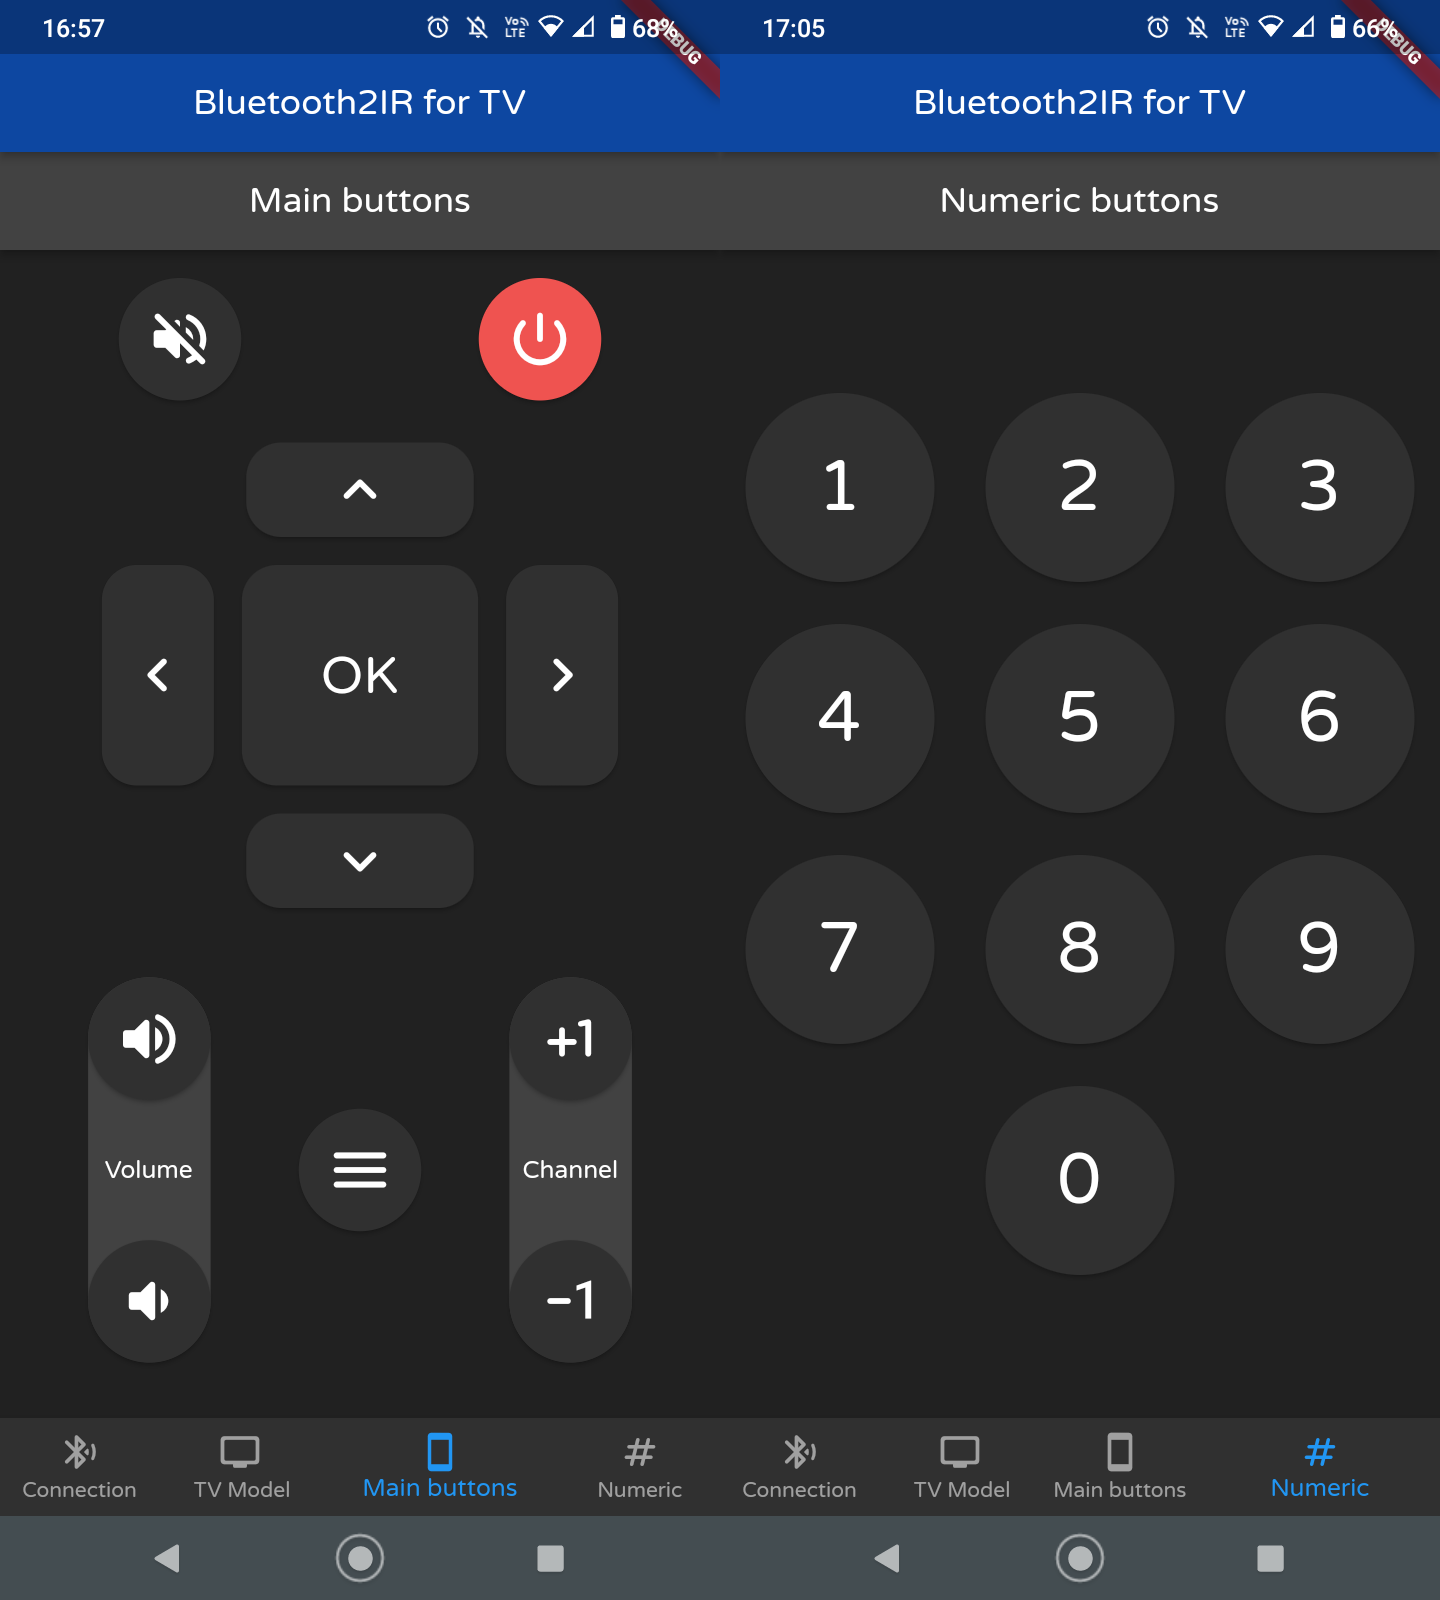
\includegraphics[width=10cm]{images/buttonScreens.png}
   \caption{Ekrany ,,Main Buttons'' oraz ,,Numeric'' aplikacji mobilnej}
   \label{Fig:buttonScreens}
\end{figure}

Każdy z przycisków po naciśnięciu wysyła dane do 2 charakterystyk serwera BLE z którym wcześniej nawiązano połączenie. Dzieje się to za pomocą metod wysyłających dane z klasy BLEService i danych typu wciskanego przycisku i kodu sygnału podczerwonego zależnych od wybranego modelu telewizora, którym użytkownik chce sterować. Funkcja przypisana do parametru onPressed przycisku numerycznego ,,1'', wysyłająca te dane dla tego przycisku, została przedstawiona na List. \ref*{Lst:buttonSend}.

\lstinputlisting[inputencoding=utf8/cp1250, language={C++}, caption={\protect\input{captions/buttonSend.txt}\protect\relax}, label={Lst:buttonSend}]{codes/buttonSend.cpp}
\clearpage



\section{Testy i prezentacja finalnego systemu}
\subsection{Ustanawianie połączenia aplikacji z urządzeniem}
Aplikacja mobilna podczas uruchomiania pyta użytkownika czy nie chce on włączyć adaptera Bluetooth i lokalizacji jeśli te nie są już włączone. Niweluje to możliwość ślepych prób odświeżania dostępnych urządzeń w poszukiwaniu urządzenia pośredniczącego. Jeżeli mikrokontroler jest zasilony, a aplikacja ma włączone oba wymagne moduły w ciągu 3 sekund od odświeżenia listy dostępnych urządzeń jest znajdowany system pośredniczący. Teraz użytkownik może połączyć się z nim za pomocą pojedynczego kliku na wyświetlanej liście w aplikacji. Stan urządzenia pośredniczącego i aplikacji mobilnej na chwilę przed nawiązaniem połączenia przedstawia Rys. \ref*{Fig:scanTest}.

\begin{figure}[ht]
   \centering
   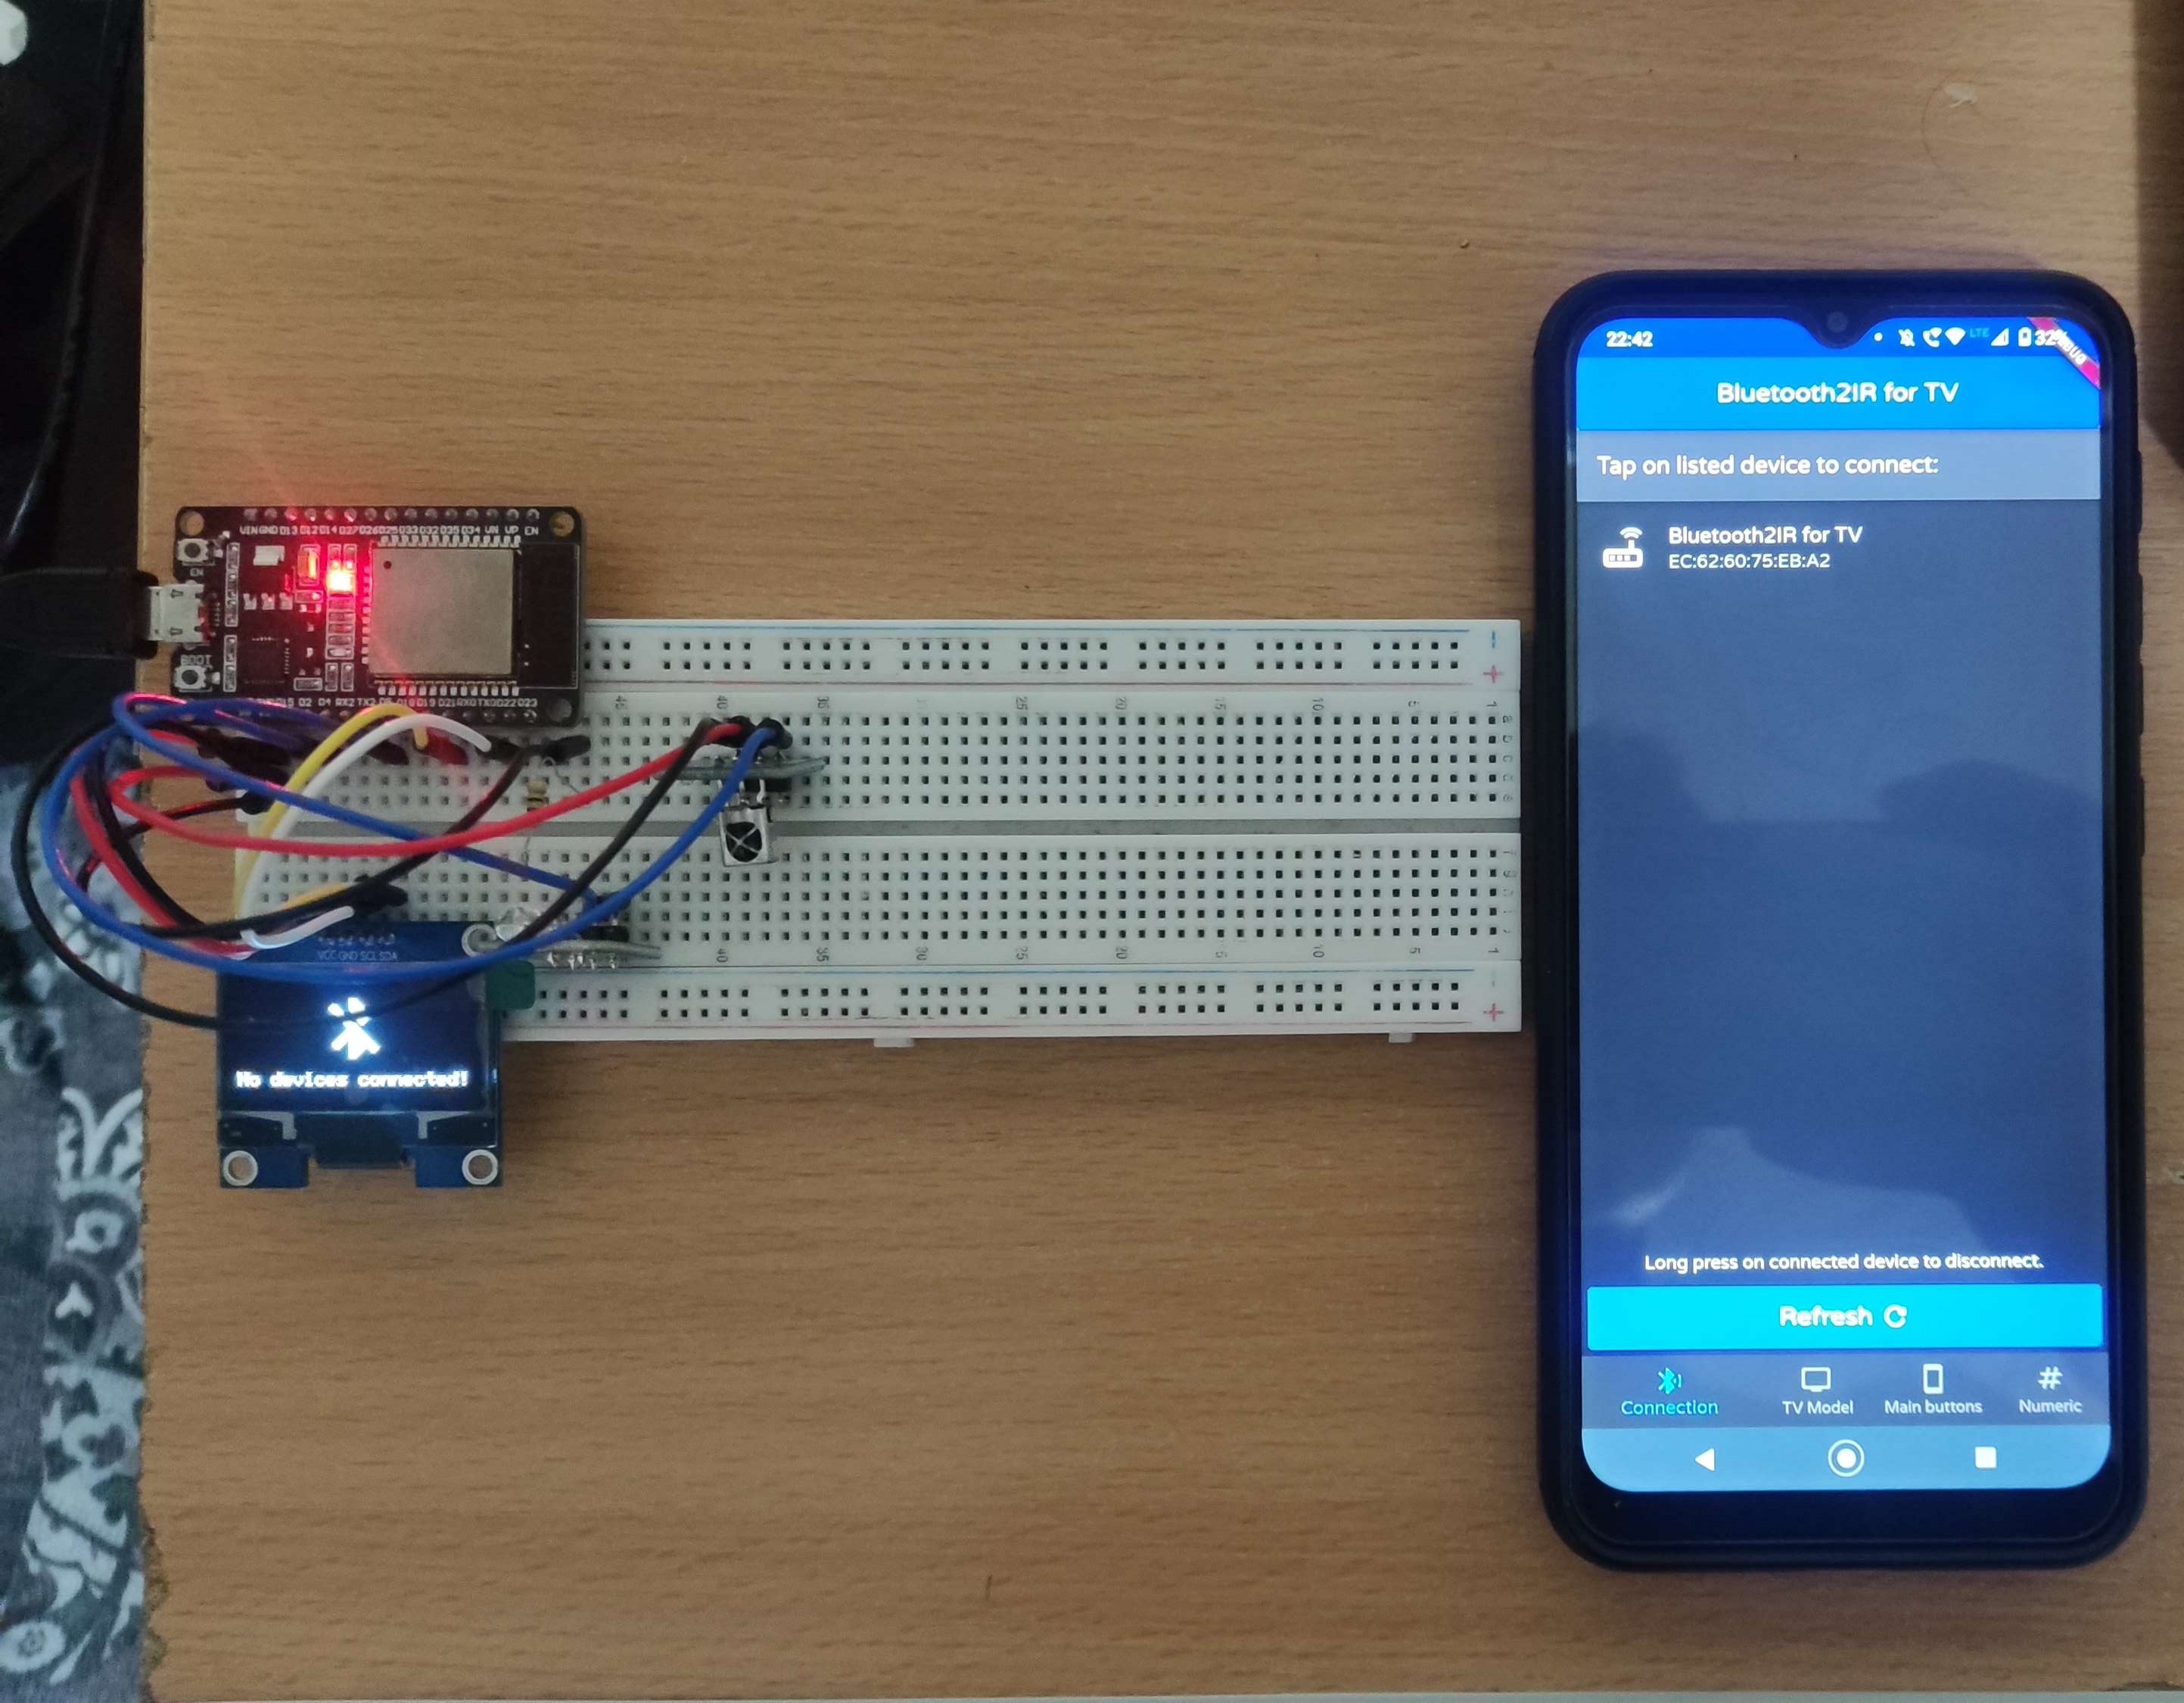
\includegraphics[width=14cm]{images/scanTest.jpg}
   \caption{Stan systemu po włączeniu zasilania w urządzeniu pośredniczącym i wykonaniu skanowania dostępnych urządzeń w aplikacji mobilnej}
   \label{Fig:scanTest}
\end{figure}

Nawiązywanie połącznia aplikacji z systemem wysyłającym sygnały podczerowne do telewizora trwa zazwyczaj do 3 sekund. Jeżeli ten czas jest przekroczony oznacza to zazwyczaj niski poziom naładowania baterii lub spadek napięcia zasilającego mikrokontroler. Po połączeniu się za pomocą BLE obu elementów systemu sterowania telewizorem, na wyświetlaczu OLED widać zwiększenie się liczby połączonych urządzeń, a w aplikacji połączone urządzenie jest podświetlane na zielono. Stan obu urządzeń po nawiązaniu połączenia przedstawia Rys.\ref*{Fig:connectingTest} Tak połączony system, można teraz parametryzować w kolejnym oknie aplikacji.
\begin{figure}[ht]
   \centering
   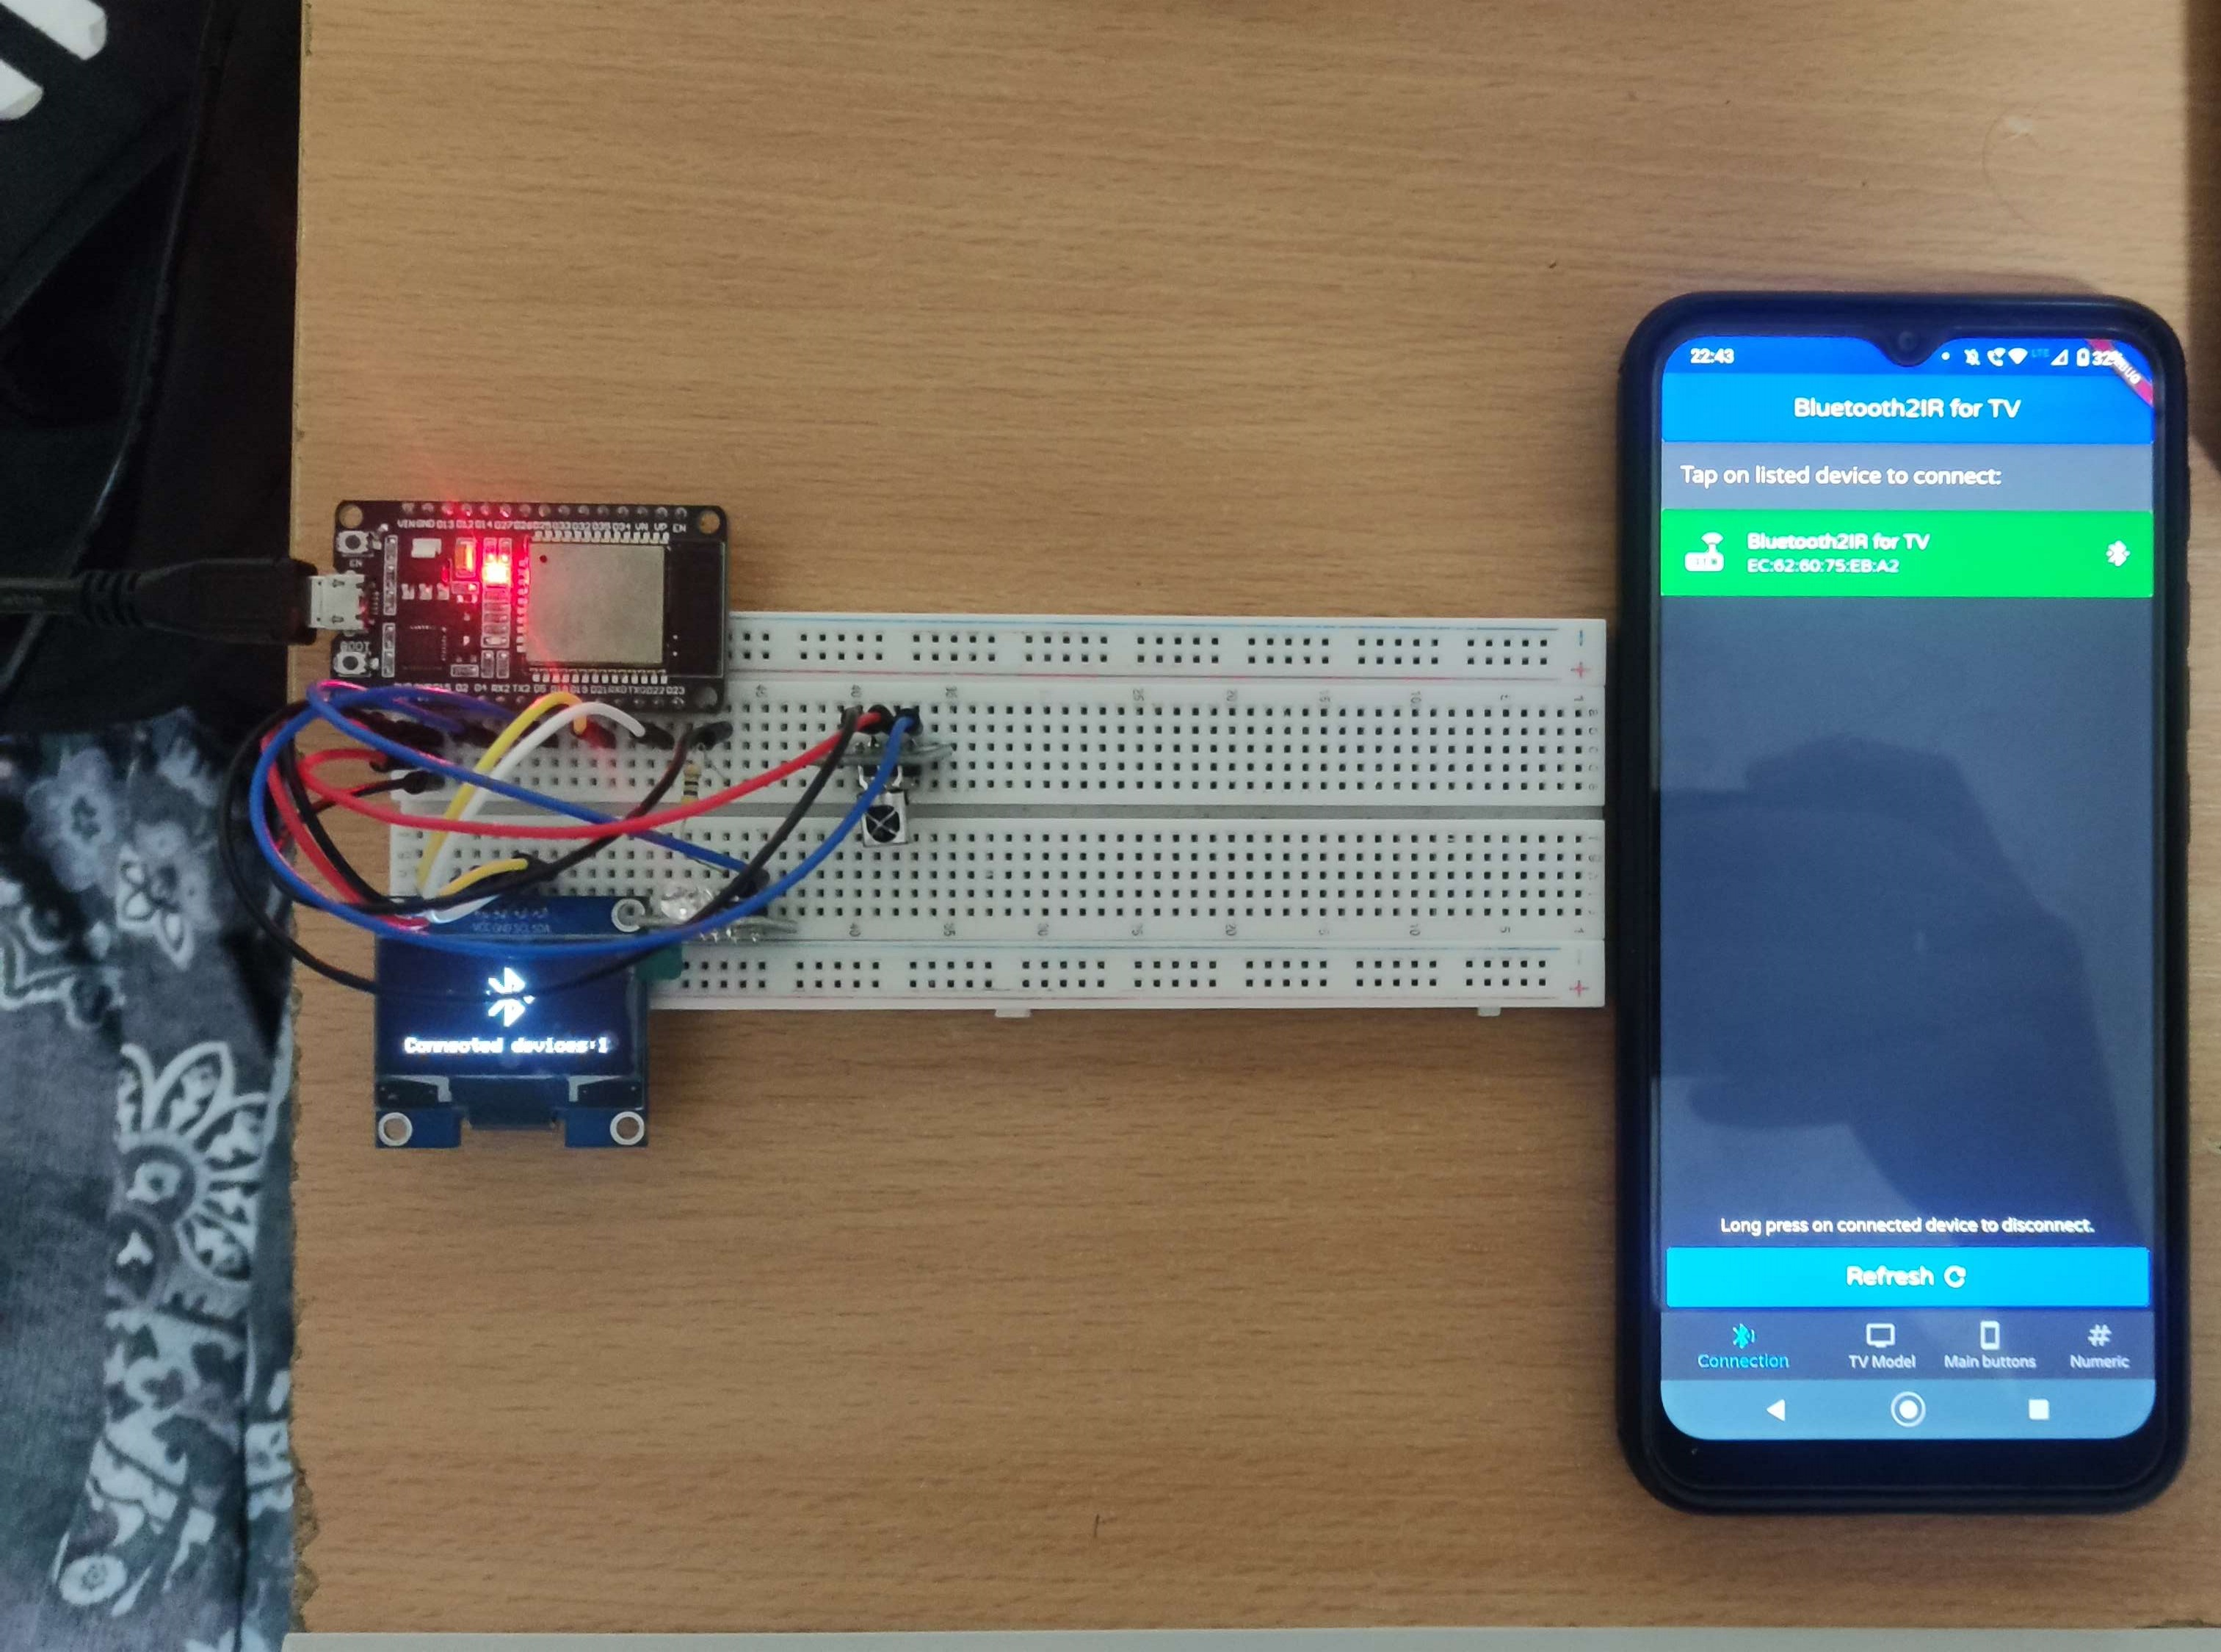
\includegraphics[width=14cm]{images/connectingTest.jpg}
   \caption{Stan systemu po nawiązaniu połączenia}
   \label{Fig:connectingTest}
\end{figure}

\subsection{Edycja i wybór modelu telewizora w aplikacji}
Przechodząc do ekranu ,,TV Model'', nie zobaczy się od razu listy dostępnych predefiniowanych lub zdefiniowanych przez użytkownika telewizorów którymi można sterować lecz będzie to opóźnione o kilka sekund z uwagi na konieczność wczytania tych modeli z pamięci apliakacji. Po pierwszym wczytaniu danych z pamięci ekran działa już płynnie i pozwala na swobodne działanie.

Użytkownik nie jest zmuszony do definiowania własnego modelu telewizora. Może on wybrać z dostępnej listy model marki Manta i przejść bezpośrednio do ekranów aplikacji z przyciskami pilota i sterować swoim urządzeniem telewizyjnym.

Jeśli jednak chce edytować już wcześniej utworzony przez siebie model urządzenia odbierającego sygnały podczerwone najlepiej, żeby zaopatrzył się w kody sygnałów IR interesującego go modelu z materiałów producenta. Może jednak skorzystać też z czytnika kodów podczerownych oprogramowanego w urządzeniu pośredniczącym. Wystarczy, że skieruje on swojego starego pilota na to urządzenie i będzie wciskać przyciski. Działanie to zaprezentowano na Rys. \ref*{Fig:irCodeRemote}.

\begin{figure}[ht]
   \centering
   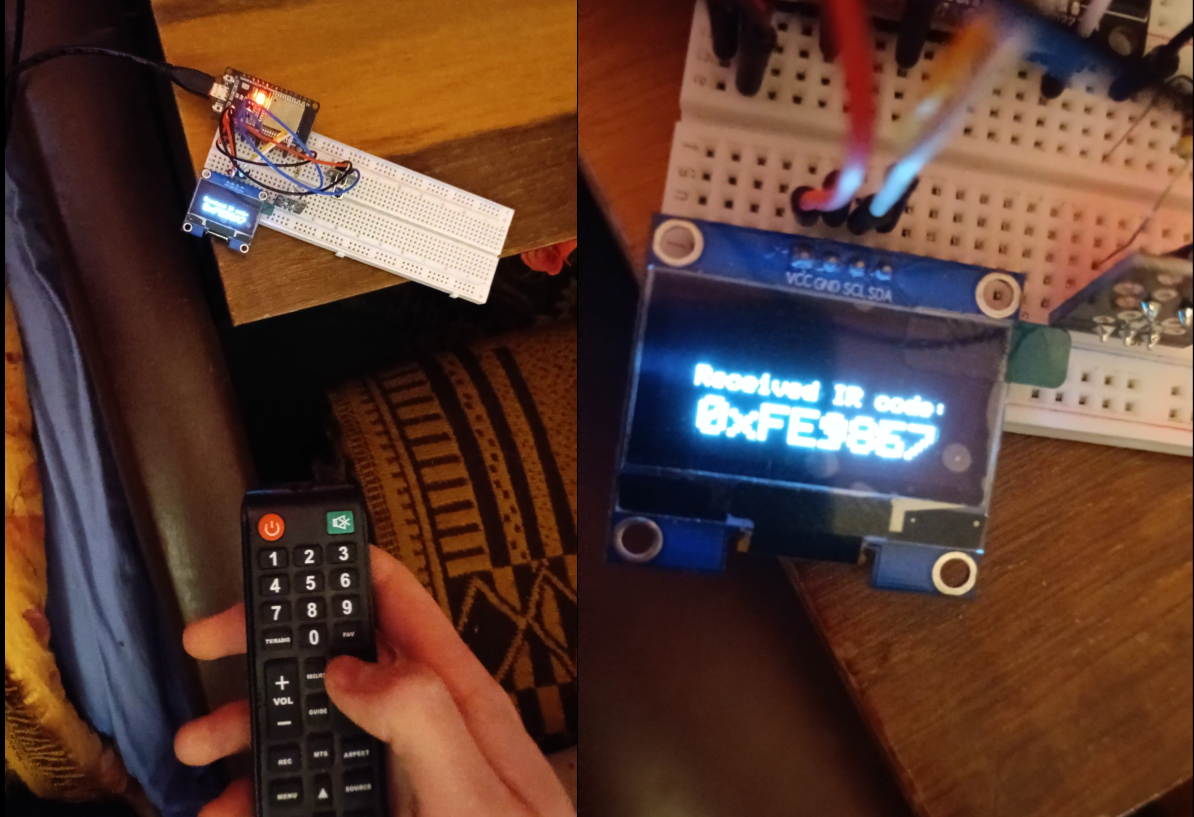
\includegraphics[width=14cm]{images/irCodeRemote.png}
   \caption{Stan wyświetlacza OLED po odebraniu kodu IR z przycisku zwiększenia głośności pilota do telewizora ,,Manta''}
   \label{Fig:irCodeRemote}
\end{figure}

 Otrzymane w ten sposób szesnastkowe kody IR na ekranie wyświetlacza OLED, użytkownik może zapisać do odpowiednich pól syngałów podczerownych w aplikacji mobilnej wybranego zdefiniowanego przez niego zestawu. Aplikacja sprawdza przed ich zapisaniem jednak poprawność tych kodów oraz czy nie zmieniane są predefiniowane modele. W razie potrzeby podpowiada użytkownikowi jaki popełnił błąd lub infromuje go o innych możliwościach działania.

 Nasłuchując syngałów IR pochodzących z pilota do telewizora marki ,,Manta'' zebrano wszystkie kody przycisków pilota zawartych na kolejnych ekranach apliakacji mobilnej. Zebrane kody szesnastkowe zapisano w kodzie aplikacji i utoworzono z nich opisywany już predefiniowany zestaw przycisków dla tego telewizora, którego użtykownik nie może usunąć z listy.

\subsection{Korzystanie z przycisków pilota}
Kiedy użytkownik ustawił już swój model telewizora w aplikacji oraz nawiązał połączenie BLE z urządzeniem pośredniczącym może już korzystać z przycisków pilota w aplikacji mobilnej. Reakcja odbiornika na wciśnięty przycisk jest właściwie natychmiastowa i użytkownik jej nie odczuwa. Sam pilot nie obsługuje jednak przytrzymywania przycisku, co może stać się zaletą ponieważ nie możliwe w ten sposób jest wysyłanie masy sygnałów naraz co często ma niezamierzone skutki jak zbyt duże zwiększenie głośności urządzenia. Na Rys. \ref*{Fig:buttonsTest} przedstawione zostało użycie przycisku wyciszającego telewizor oraz przycisków numerycznych do podania numeru kanału.

\begin{figure}[ht]
   \centering
   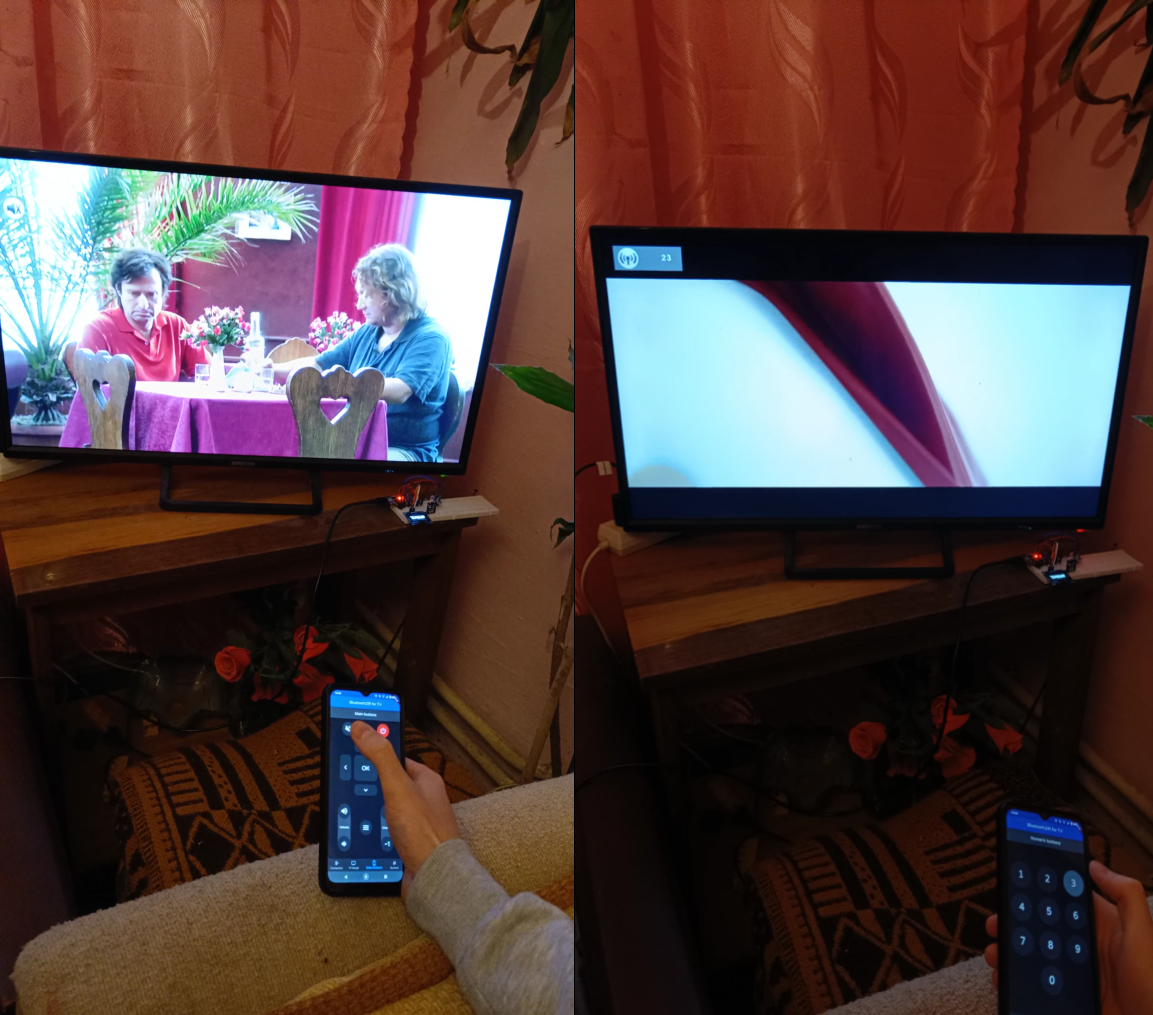
\includegraphics[width=13cm]{images/buttonsTest.png}
   \caption{Wciśnięcie przycisku wyciszenia i wpisanie numeru kanału w aplikacji mobilnej pilota}
   \label{Fig:buttonsTest}
\end{figure}

Z sterowania telewizorem może korzystać wiele aplikacji mobilnych jednocześnie dzięki zastosowania serwera BLE na urządzeniu pośredniczącym. Dlatego klient ciągle połączony z serwerem nie blokuje możliwości sterowania tym urządzeniem mutlimedialnym dla innych użytkowników domowych.

\clearpage

\section{Zakończenie}

Niniejsza praca miała na celu zaproponowanie rozwiązania sterowania telewizorem z poziomu smartfona dzięki aplikacji mobilnej i urządzenia pośredniczącego opartego o mikrokontroler z niezbędnymi modułami. Przedstawiono w niej i omówiono technologie i koncepty, z których skorzystano podczas procesu projektowania tego systemu. Opisane zostały też najważniejsze elementy fizycznej części systemu oraz oprogramowanie mikrokontrolera i zbudowana aplikacja mobilna oraz ich współpraca w sterowaniu telewizorem.

Utworzony prototyp systemu zapewnił możliwość programowani przycisków pilota w aplikacji mobilnej w oparciu o szesnastkowe kody syngałów podczerwonych. Kody te można uzyskać przeglądając sieć i strony producentów urzadzeń multimedialnych oraz dzięki wbudowanemu w urządzenie pośredniczące czytnikowi kodów IR, który po odebraniu takowego wyświetla go na ekranie OLED. Za pomocą skorzystania z serwera BLE zapewniono także dostęp do systemu dla wielu użytkowników jednocześnie. Utworzona aplikacja mobilna jest prosta w użytkowaniu i intuicyjna nawet dla użytkowników nieobytych z technologią obecną w dzisiejszych smartfonach.

Zaprojektowany prototypowy system aplikacji mobilnej i urządzenia pośredniczącego opartego o mikrokontroler jest już w pełni funkcjonalny i może zostać przekształcony do produktu komercyjnego. Aby zwiększyć jednak jego atrakcyjność na rynku można wskazać kilka usprawnień, jak:
\begin{itemize}[label=-,labelsep=0.4cm,leftmargin=0.6cm]
   \item zabudowanie urządzenia pośredniczącego w wygodną prostokątną obudowę z odpowiednim rozłożeniem modułów
   \item wprowadznie automatyzacji programowania kodów IR i wczytywania ich z plików JSON
   \item dodanie obługi inteligentnych gestów w aplikacji dla konkretnych typów urządzeń
   \item wprowadzenie kreatora ekranów przycisków w aplikacji dla maksymalnej uniwersalności rozwiązania
   \item wprowadzenia logowania użytkowników aby przechowywać ustawienia w wygodny dla niego sposób na serwerze
   
\end{itemize}

Autor za własny wkład pracy uważa: 

\clearpage
\addcontentsline{toc}{section}{Literatura}
\bibliography{biblgr}
\bibliographystyle{plain}

\clearpage

\makesummary

\end{document}
